\documentclass[]{interact}

\usepackage[sort]{natbib}% Citation support using natbib.sty
% \bibpunct[, ]{(}{)}{;}{a}{,}{,}% Citation support using natbib.sty
% \renewcommand\bibfont{\fontsize{10}{12}\selectfont}

\usepackage{amssymb}
\usepackage{amsmath}


%% The lineno packages adds line numbers. Start line numbering with
%% \begin{linenumbers}, end it with \end{linenumbers}. Or switch it on
%% for the whole article with \linenumbers.
\usepackage{lineno}

% \usepackage[backend=biber,natbib=true]{biblatex}

\usepackage{eurosym}
\usepackage{booktabs}

\usepackage{tabularx}
\usepackage{longtable}
\usepackage{xltabular}
\usepackage[table]{xcolor}

\usepackage{wrapfig}

% \usepackage{appendix}

\usepackage{epstopdf}% To incorporate .eps illustrations using PDFLaTeX, etc.
\usepackage[caption=false]{subfig}% Support for small, `sub' figures and tables
%\usepackage[nolists,tablesfirst]{endfloat}% To `separate' figures and tables from text if required
%\usepackage[doublespacing]{setspace}% To produce a `double spaced' document if required
%\setlength\parindent{24pt}% To increase paragraph indentation when line spacing is doubled

% \usepackage[sort]{natbib}% Citation support using natbib.sty
\bibpunct[, ]{(}{)}{;}{a}{,}{,}% Citation support using natbib.sty
\renewcommand\bibfont{\fontsize{10}{12}\selectfont}% To set the list of references in 10 point font using natbib.sty
\bibliographystyle{abbrvnat}

%\usepackage[natbibapa,nodoi]{apacite}% Citation support using apacite.sty. Commands using natbib.sty MUST be deactivated first!
%\setlength\bibhang{12pt}% To set the indentation in the list of references using apacite.sty. Commands using natbib.sty MUST be deactivated first!
%\renewcommand\bibliographytypesize{\fontsize{10}{12}\selectfont}% To set the list of references in 10 point font using apacite.sty. Commands using natbib.sty MUST be deactivated first!

\theoremstyle{plain}% Theorem-like structures provided by amsthm.sty
\newtheorem{theorem}{Theorem}[section]
\newtheorem{lemma}[theorem]{Lemma}
\newtheorem{corollary}[theorem]{Corollary}
\newtheorem{proposition}[theorem]{Proposition}

\theoremstyle{definition}
\newtheorem{definition}[theorem]{Definition}
\newtheorem{example}[theorem]{Example}

\theoremstyle{remark}
\newtheorem{remark}{Remark}
\newtheorem{notation}{Notation}

\begin{document}
\title{Sustainable optimal reliability for engineering structures}

%% use optional labels to link authors explicitly to addresses:
\author{\name{Jelle Knibbe\textsuperscript{a,b}, Raphaël Steenbergen\textsuperscript{b,c}, Pieter van Gelder\textsuperscript{a}, Amir Pooyan Afghari\textsuperscript{a}}
\affil{\textsuperscript{a}Faculty of Technology, Policy and Management, Delft University of Technology,  Jaffalaan 5, Delft, the Netherlands; 
\textsuperscript{b} Department of Reliable Structures, Netherlands Organisation for Applied Scientific Research (TNO), Molengraaffsingel 8, Delft, the Netherlands; 
\textsuperscript{c}Faculty of Engineering and Architectures, Ghent University, Jozef Plateaustraat 22, Ghent, Belgium}}

%% Abstract, max 250 words!

\maketitle

\begin{abstract}
%% Text of abstract

This paper presents a novel approach towards deriving optimal reliability for engineering structures.
Currently, this is based on life cycle monetary optimisation, using a cost function dependent on the design of a structure, its failure probability and obsolescence rate.
This paper proposes augmenting this cost function with a shadow-costed emissions function, such that the optimal reliability is influenced by social environmental aspects as well as monetary ones, allowing decision-makers to take a broader view on this crucial aspect of structural design.
This new approach is demonstrated with a case study based on a typical structural design, where applying the emission-augmented cost function reduces the optimal reliability index by 0.12 compared to the conventional approach.
This result is sensitive to the shadow price used to commensurate cost and emissions, with a larger shadow price or larger environmental impact relative to cost resulting in a larger reduction.
Alternatively, the optimisation can also be performed using either the cost or emission function, with the other as a constraint.
The threshold value for this constraint then sets the optimal reliability index.
Furthermore, both optimal reliability values are also sensitive to the costs incurred when the structure fails, the degree of uncertainty in the loads on and resistance of the structure, and the general design conditions of the structure.
However, the difference between the conventional and augmented optimal reliability is less affected by these aspects.




\end{abstract}



%% Keywords
\begin{keywords}
%% keywords here, in the form: keyword \sep keyword
Structural safety; Optimal reliability; Shadow costs; Sustainability
%% PACS codes here, in the form: \PACS code \sep code

%% MSC codes here, in the form: \MSC code \sep code
%% or \MSC[2008] code \sep code (2000 is the default)

\end{keywords}

%% Add \usepackage{lineno} before \begin{document} and uncomment 
%% following line to enable line numbers
\linenumbers

%% main text
%%

\section{Introduction}


The construction industry contributes more than 10\% of the GDP of many countries \citep{RILEM2022GLOBEEnvironment}, along with 20\% of global CO\textsubscript{2} emissions \citep{Huang2018CarbonSector}.
From both economic and environmental viewpoints, there is therefore much to gain by optimising structural designs in terms of minimal costs and emissions, while ensuring they are safe enough from a societal point of view.
Decision makers in the field of structural engineering, such as designers, code committees, or asset managers, benefit from guidance on this optimisation.
As such, a crucial question from their perspective is the appropriate level of reliability for a structure, in other words, \emph{how safe should a structure be?}
The answer to this question then informs decisions on structural design.
To find it, the costs, risks, and benefits of a structure need to be considered, ideally in the broad sense, including environmental impacts and societal risks due to the structure potentially failing and causing harm to its users.
These aspects can be quantified through life cycle analyses, taking all three `pillars' of sustainability into account \citep{Knibbe2026PlaceHolder, Valdivia2021PrinciplesAssessment}.
The level of reliability corresponding to the best `performance' over the life cycle of the structure can then be considered as an appropriate design target for decision makers.

This level can be numerically represented by the target failure probability $P_{f,target}$ or, equivalently, the target reliability index $\beta_{target}$.
These are linked through the following conversion:
\begin{equation}
\label{eqn:beta_Pf}
    \beta = \Phi^{-1}(1-P_f)
\end{equation}
Where $\Phi^{-1}(\cdot)$ is the inverse of the cumulative distribution function of a standard-normal distributed random variable.
Current norms on target reliabilities \citep{iso2394, EN1990} distinguish optimal and acceptable reliability values \citep{Fischer2019OptimalDesign}, noted here as $\beta_{opt}$ and $\beta_{acc}$ respectively, where the most stringent value forms the target reliability:
\begin{equation}
    \beta_{target} = \max(\beta_{opt}, \beta_{acc})
\end{equation}
The optimal value is found by minimising a lifetime cost function, and the acceptable value through the minimal required investment to ensure adequate life safety.
This current framework has been developed based on the work of several authors in the field of structural safety, including \citep{Rackwitz2000OptimizationVerification, Rackwitz2006TheCriteria, Rackwitz2008TheVerification, Viljoen2012DerivingLQI, Fischer2019OptimalDesign, Pandey2004LifeSafety, Pandey2024LifeStructures}.
At present, however, the cost functions used to determine both $\beta_{opt}$ and $\beta_{acc}$ are based on monetary considerations only.
Environmental concerns are not accounted for, which is undesirable considering the aforementioned impact of construction on the environment and the societal urgency of mitigating climate change.
If the construction sector is to contribute to this mitigation, decision-makers require an approach for determining target reliabilities that \emph{does} take environmental impacts into account.
Such an approach is presented in this paper, focusing on optimal reliabilities.
This builds upon previous work by the same authors, focused on acceptable reliability \citep{Knibbe2026PlaceHolder}. 

Sections 2 and 3 present the current approach for finding optimal reliability values, and expand on the need for further development from social and environmental perspectives.
This serves as background to Section 4, where the augmented approach itself is presented, followed by a demonstration through a typical case study in Section 5.
Section 6 contains an analysis of the case study results, and the impact of the presented approach with respect to the conventional approach.
Finally, Section 7 provides a conclusion and a brief discussion.

\newpage
\section{Optimal Reliability}

In the ISO 2394 norm on structural reliability \citep{iso2394} and the probabilistic model code by the joint committee on structural safety \citep{JCSS2000ProbabilisticDesign}, optimal reliability values are based on a cost function derived from the infinite renewal model of Rackwitz \citep{Rackwitz2000OptimizationVerification}, formulated as follows:
\begin{equation}
    \label{eqn:C_total}
    C_{total}(x) = C_{const}(x) + C_{const}(x) \frac{\omega}{\gamma} + (C_{const}(x) + C_H) \frac{P_f(x)}{\gamma}
\end{equation}
This quantifies the total lifetime monetary costs of a generic structure as a function of a decision parameter $x$ representing the structural design, with future costs discounted towards their net present value (NPV).
This consists of three components:

\begin{itemize}
    \item The initial construction costs $C_c = C_{const}(x)$, which are incurred once at the beginning of the lifetime of the structure. 
    \item The obsolescence costs $C_o = C_{const}(x)\frac{\omega}{\gamma}$, representing the structure being replaced with a yearly obsolescence rate $\omega$, incurring the construction costs again.
    These yearly costs are discounted using the yearly exponential discount rate $\gamma$ \citep{Green1996ExponentialTime}.
    \item The failure costs $C_f = (C_{const}(x) + C_H) \frac{P_f(x)}{\gamma}$, where $P_f(x)$ is the \emph{yearly} failure probability and $C_H$ are the additional damage costs incurred at failure, in addition to the construction costs for replacing the structure.
\end{itemize}

A linear function for $C_{const}(x)$ is often assumed, though this is not strictly necessary:
\begin{equation}
    \label{eqn:C_const_linear}
    C_{const}(x) = C_0 + C_1 x
\end{equation}
Where $C_0$ are costs independent of the decision variable, and $C_1$ represents the costs varying linearly with $x$.
Non-linear formulations could be used for $C_{const}(x)$ as well, as well as functions with multiple decision variables ($C_{const}(\mathbf{x})$), though these are rarely encountered in literature.
In general, $C_{const}(x)$ should be monotonically increasing. %($\frac{dC_{const}}{dx} \geq 0$ for all $x$).

The failure probability $P_f(x)$ is calculated through a reliability analysis, based on a limit state function $Z=g(x,\mathbf{R})$ and a set of random variables $\mathbf{R}$ with joint distribution $f_{\mathbf{R}}(\mathbf{r})$.
For a given value of the decision variable $x=x^*$, the failure probability is given by $P_f(x) = P[Z<0|x=x^*]=P[g(x^*,\mathbf{R})<0]$, together forming a probabilistic model of the structure.
For elementary limit state functions and probabilistic models \citep{Rackwitz2000OptimizationVerification}, an analytical expression of the failure probability may be available.
Otherwise, evaluating $P_f(x)$ requires a method such as FORM or Monte Carlo \citep{Ditlevsen2005StructuralMethods}.
% Generally, for increasing $x$, $P_f(x)$ should decrease with a decreasing slope ($\frac{dP_f}{dx} < 0$ and $\frac{d^2P_f}{dx^2} > 0$).

The definition of the decision variable $x$ is flexible.
In some literature, $x$ represents the ratio between the mean resistance of the structure $\mu_R$ and the mean load $\mu_S$ imposed on it ($x=\mu_R/\mu_S$) \citep{Rackwitz2000OptimizationVerification, Viljoen2012DerivingLQI}.
Less abstract quantities such as the section modulus of a beam are used as well \citep{Hingorani2023TowardsDesign}.

The optimal failure probability is found by minimising the cost function with respect to $x$, yielding the optimal value $x_{opt}$ and associated $P_{f,opt} = P_f(x_{opt})$ and $\beta_{opt}$:
\begin{equation}
    \begin{aligned}
        x_{opt} = \arg \min_{x} C_{total}(x)\\
    \end{aligned}
\end{equation}
Figure \ref{fig:generic_cost_Pf} visualises the optimisation problem.
Assuming the common linear formulation for $C_{const}$ is used, the parameter $C_1$ has a major influence on the optimal reliability: the larger it is, the more expensive additional reliability becomes, and the more the optimal failure probability is `pushed' upwards (for other formulations, any parameter influencing the positive slope of $C_{const}$ plays a similar role).
Similarly, the damage cost $C_H$ (which is generally much larger than $C_{const}(x)$ at the optimum) dominates the failure costs $C_f$ and `pulls' the optimal failure probability downwards.
This `push-pull' effect plays an important role in determining the optimal reliability of a structure, and becomes clear in the current norms.
ISO2394 defines three cost classes and three consequence classes by the relative magnitude of $C_1$ and $C_H$, respectively, and the combination of these classes determines the optimal reliability.
% In some literature \citep{Fischer2019OptimalDesign, Steenbergen2018TargetMaking}, the classes are defined by the ratio of $C_1$ and $C_H$ respectively to $C_0$ or $C_{const}$.
% A larger (relative) $C_H$ prescribes a larger $\beta_{opt}$ and smaller $P_{f,opt}$, while a larger $C_1$ causes the opposite.
Table \ref{tab:iso_table} presents these nine combinations, and thereby represents the current status quo for optimal reliability.



\begin{table}[h!]
    \caption{Conventional optimal failure probabilities, from \citep{iso2394}}
    \centering
    \begin{tabular}{c|lccc}
        Cost & &  \multicolumn{3}{c}{Consequence classes $C_H/C_0$}\\
        $C_1/C_0$ & & Minor & Moderate & Major\\ \hline
        
        Large & $\beta_{opt}$ &  3.1&  3.3& 3.7\\
          &$P_{f,opt}$& $10^{-3}$& $5 \cdot 10^{-4}$&$10^{-4}$\\ \hline
          
        Normal &$\beta_{opt}$ & 3.7 & 4.2 & 4.4\\
          &$P_{f,opt}$& $10^{-4}$& $10^{-5}$&$5\cdot10^{-6}$\\ \hline
        
        Small &$\beta_{opt}$ & 4.2 & 4.4 & 4.7\\
          &$P_{f,opt}$& $10^{-5}$& $5\cdot10^{-6}$&$10^{-6}$
    \end{tabular}    
    \label{tab:iso_table}
\end{table}


\begin{figure}[h]
    \centering
    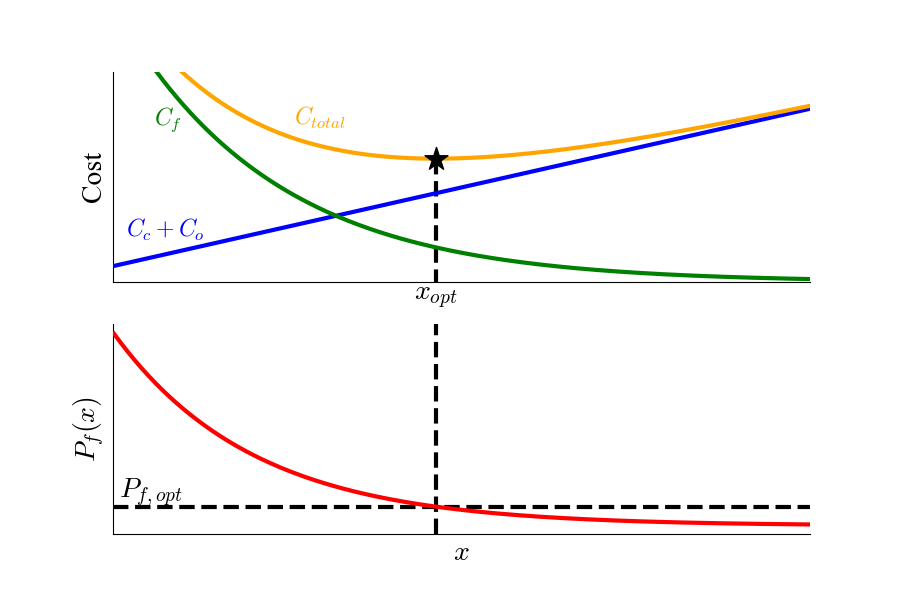
\includegraphics[width=0.95\linewidth]{Images/generic_cost_Pf.png}
    \caption{The optimisation underlying the current approach for determining optimal and acceptable reliabilities The blue line represents the `pushing' components of the cost function, and the green line the `pulling' failure costs}
    \label{fig:generic_cost_Pf}
\end{figure}






\newpage
\section{Appraisal of the current approach}
\label{sec:appraisal}

The approach for determining $\beta_{opt}$ described in the previous section can be related to the normative ethical principle of \emph{utilitarianism}: an action is morally right if it improves some measure of total societal utility \citep{Mill1863Utilitarianism, vandePoel2011EthicsEngineering}.
Given a set of possible actions, the optimal choice is the one that yields the largest utility, hence applying utilitarianism to engineering design naturally leads to solving an optimisation problem by a decision-maker.
In determining the optimal reliability of a structure, the benefit provided by the structure is generally assumed to be independent of the decision parameter $x$. 
Maximising utility is then equivalent to minimising cost (or disbenefit), and this minimisation yields the optimal reliability $\beta_{opt}$.

A prevalent criticism of utilitarianism is whether all relevant aspects of a problem can truly be captured or aggregated quantitatively within a single `utility function'\citep{vandePoel2011EthicsEngineering}. 
As mentioned previously, the optimal reliability should ideally be informed by all three `pillars' of sustainability, economic, environmental and social, to give decision-makers a broad view of the problem.
However, the current formulation of $C_{total}$ only takes monetary costs into account, so this criticism is warranted in this case.
To address it, the optimisation problem should also take environmental and societal effects into account, and not just monetary aspects.
The following addresses how this could be achieved for both `missing' pillars, and addresses a number of other ethical aspects.


\subsection{Environmental sustainability}

As mentioned in the introduction, the environmental impact of the construction sector in terms of CO\textsubscript{2}-emissions is significant.
Climate change caused by these emissions affects society as a whole, while the monetary costs are generally borne only by the owner or operator of a structure.
The current approach therefore leads to distributive injustice: the distribution of costs and benefits across stakeholders is not represented in the optimisation problem, so decision-makers cannot ensure that it remains equitable.
This is another common criticism of utilitarianism \cite{vandePoel2011EthicsEngineering}.
% If the utility function only represents the perspective of a single stakeholder, and the effects on others are ignored, the distribution of costs and benefits can become unfair even for a decision that supposedly maximises the utility.

For the environment and its importance to society to directly inform in the optimal reliability value, the societal burden (quantified as emissions) borne by the environment must also be considered as part of the utility function.
Aggregating different aspects requires them to be commensurate with each other, so that they can be summed up in a single quantity.
This is considered aggregationism, an aspect of utilitarianism taking account of multiple perspectives \citep{Narveson2009WhenWhy}, and the challenge in this approach is then how much one aspect should weigh against another, and what the role of the decision-maker is in this.
Assuming the aggregated utility function is still expressed in monetary units (e.g. euros), this means the emissions need to be `priced' in the same unit.
This `social cost of carbon' or \emph{shadow price} then represents the burden caused by emissions: economic damage, health impacts, loss of living standards, reduced opportunities for future generations \citep{Boyce2018CarbonEquity}.
It can be viewed as compensation or prevention costs for such damage, or a broader valuation of carbon emissions against monetary aspects, which also has distributional effects \cite{Shei2024DistributionalApproaches}.
Quantified values for this price therefore vary across literature, from less than 100 to several thousand dollars per ton CO\textsubscript{2} emissions \citep{Lomborg2020WelfarePolicies, Wang2022GlobalCosts, KamaliSaraji2024BridgingApplications}, also depending on worldwide policies adopted to address climate change \citep{Yang2018SocialPathways, IntergovernmentalPanelonClimateChangeIPCC2023SummaryPolicymakers}, so placing a single number on this cost is difficult.

Alternatively, instead of considering both costs and emissions in one utility function, one could be considered as a constraint in optimising the other.
This approach replaces aggregationism with sufficientarianism, an important approach for distributive justice \citep{Alcantud2022Sufficientarianism}.
A threshold value is needed instead of a carbon price: if the aspect (costs or emissions) considered as a constraint is above this threshold for a certain value of the decision variable $x$, that decision is deemed infeasible.
This constraint is considered as binary: either the disbenefit is sufficiently small, and the decision is `allowed', or the disbenefit is too large and it is not.
The feasible value of $x$ leading to the smallest value in the other objective, still forming the utility function, is then the optimum $x_{opt}$.

\subsection{Social sustainability}
The most important societal consideration in determining the target reliability is the safety of the users occupying the structure.
If the structure collapses, their lives are at risk, which should be reflected in the utility function $C_{total}$.
Intuitively, this can be expressed in the additional damage costs $C_H$, which represent the consequences of structural failure aside from replacing the structure itself.
This requires the loss of a human life to be monetarised, which is complicated from an ethical perspective, and a typical problem that arises when risks to life safety are judged using a utilitarian approach \citep{vandePoel2011EthicsEngineering}.
However, if life safety is to inform the optimal reliability, it inevitably needs to be incorporated in the decision-making problem in some manner.
In fact, a constraint based on monetarised human life safety is currently used to define the \emph{acceptable} reliability $\beta_{acc}$ following a mean life saving costs (MLSC) approach \citep{Viljoen2012DerivingLQI}.
The Life-Quality Index (LQI) is used to quantify a societal willingness to pay ($SWTP$) for saving a statistical human life \citep{Pandey2004LifeSafety}, based on the available societal resources to invest in safety improvements through GDP and life expectancy.
A minimum acceptable safety level is then derived by considering efficient safety investments to be required from a societal point of view.

This same quantity could be used as `compensation costs' for fatalities in $C_{total}$, by defining $C_H$ as follows:
\begin{equation}
    \label{eqn:C_H_SWTP}
    C_H = SWTP \cdot N_f + C_{H,other}
\end{equation}
Where $N_f$ is the expected number of fatalities should the structure fail, and $C_{H,other}$ are additional damage costs unrelated to human safety.
Some literature uses a similar formulation \citep{Hingorani2023TowardsDesign}, but it is not explicitly mandated in ISO2394 \citep{iso2394} (appendix G) or the JCSS model code \cite{JCSS2000ProbabilisticDesign} (section 7) for \emph{optimal} reliability.
In fact, ISO2394 notes the possibility of the optimal reliability being unacceptable from the perspective of life safety ($\beta_{acc} > \beta_{opt}$).
Using the above formulation for $C_H$, however, ensures that this does not occur \citep{Fischer2019OptimalDesign} ($C_H \geq SWTP \cdot N_f$ leads to $\beta_{opt} \geq \beta_{acc}$).
On the other hand, if human live safety is disregarded in the optimisation (i.e. by defining $C_H = C_{H,other}$), their value is implicitly placed at zero.
For many residential and commercial structures, loss of human life is the most important factor in the consequences of structural failure, so $C_{H,other}$ will often be much smaller than $SWTP \cdot N_f$, or even negligible compared to it.
In that case, $\beta_{opt}$ \emph{will} be notably smaller than $\beta_{acc}$, and the risk to the users of the structure would thus be too large for one criterion while being disregarded in the other.
This would again be inadmissible from the perspective of distributive justice \citep{vandePoel2011EthicsEngineering}.

Furthermore, the two reliability criteria of $\beta_{acc}$ and $\beta_{opt}$ have somewhat different interpretations.
The LQI-based criterion only provides an acceptable lower bound on the reliability index $\beta$, but does not state whether a value larger than this threshold could be of merit \citep{Fischer2019OptimalDesign}.
To answer this, the optimal reliability criterion is considered, but it would then not be useful to decision makers if it consistently yielded smaller reliabilities than the acceptable value.
Rather, $\beta_{opt}$ should reflect potential advantages to exceeding the lower bound of $\beta_{acc}$.
This will generally be the case if $C_H \geq SWTP \cdot N_f$, as noted above, where $C_{H,other}$ then sets these advantages in terms of expected damage costs being reduced by further decreasing $P_f$.
So, to allow the advantages of further increasing reliability beyond the acceptable minimum to be considered by decision-makers, and to avoid the implicit neglect of human life safety leading to unacceptable `optimal' values, this formulation of Equation \ref{eqn:C_H_SWTP} for $C_H$ should be used, despite ethical trepidations in monetarising human lives.

% Taking human life risks into account covers an important aspect of social sustainability.
% The norm ISO14075 \cite{ISO14075} on social life cycle assessment contains a number of other social aspects which should be taken into account in engineering design, such as accessibility, adaptability and cultural heritage. 
% These are important, but generally not directly affected by structural reliability, the design aspect considered in this paper.
% Because of this, they are not further considered here, and the remainder of this work focuses on involving environmental sustainability in the optimal reliability approach, while accepting the above monetarisation of human life risk.

\subsection{Towards an improved framework}

Considering the points above, an improved method for finding optimal reliability should ensure that life safety end environmental impact. are taken into account in the optimisation problem.
The former can be achieved by ensuring that $C_H$ includes fatality compensation costs, by mandating a formulation such as Equation \ref{eqn:C_H_SWTP}.
This does not require the framework of optimising $C_{total}$ and the LQI-based acceptance criterion to be fundamentally altered, though $\beta_{acc}$ and $\beta_{opt}$ can be interpreted slightly differently, with the acceptance criterion giving a lower bound on the reliability and the optimal value representing the potential utility of exceeding this lower bound.

Including emissions requires more development. 
The optimisation problem inherently needs to be augmented with a second objective function representing the emissions.
The next section proposes how this function can be formulated, and how the optimisation problem can then be solved through either aggregationism or sufficientarianism, resulting in a single optimal value.




% Needs to be usable, so similar format as status quo

% Take emissions into account


% (discounting later)

\section{A proposed augmentation to the optimal reliability approach}
\label{sec:proposed_emission}

The augmentation to the conventional approach for determining optimal reliability values is presented.
The aim is to convert the single-objective monetary optimisation problem into a two-objective problem, with the second objective being environmental emissions, and then find a single optimal solution.
The primary approach towards finding this solution will be to apply shadow costing to the emissions.
To facilitate this, an expression for the emissions is used which is similar to that of the costs, following the renewal model by \citep{Rackwitz2000OptimizationVerification}:
\begin{equation}
    \label{eqn:E_total}
    E_{total}(x) = E_{const}(x) + E_{const}(x) \frac{\omega}{\gamma} + (E_{const}(x) + E_H) \frac{P_f(x)}{\gamma}
\end{equation}
Where $E_{total}$ is the lifetime CO\textsubscript{2}-equivalent emissions, given in kilograms (kg CO\textsubscript{2}eq), varying with the same decision variable $x$ as in $C_{total}$.
The emissions are discounted so that the shadow cost is given as the net present value, which is needed to formulate it commensurate with the conventional costs $C_{total}$ (also given in NPV).
This similar formulation of  $C_{total}$ and $E_{total}$ allows the proposed method to be integrated in existing codes, and to compare the two objective functions directly, as both contain the aforementioned `push-pull' effect.
Some literature suggests that emissions and costs should not be discounted in the same way, as the change in valuation over time (represented by discounting) differs for economic and environmental aspects.
For simplicity, a single discount factor $\gamma$ is used here, but the possibility of differential discounting is suggested for future research.

Similarly to the monetary cost function, the total emissions can be split in the construction emissions $E_c=E_{const}(x)$, obsolescence emissions $E_o=(E_{const}(x)\frac{\omega}{\gamma})$ and failure emissions $E_f=(E_{const}(x)+E_H)\frac{P_f(x)}{\gamma}$.
A linear formulation could be used for $E_{const}(x)$ as is often done for $C_{const}$:
\begin{equation}
    \label{eqn:E_const_lin}
    E_{const}(x) = E_0 + E_1 x 
\end{equation}
In this formulation, the constant emissions $E_0$ represent the emissions produced by the transport of structural components or other sources independent of $x$, for example, while the variable emissions $E_1$ are the emissions caused by producing the structural material used in the components.

% The additional failure emissions $E_H$ are expected to be small compared to $E_{const}$, especially when compared to the same ratio in the cost model.
% Structural failure, by itself, does not cause much greenhouse gas emissions outside of replacement of the structure, which is already represented in $E_{const}$ in the failure term.
% The effects of this will become clear in the case study presented in the next section.

\subsection{Primary approach: shadow-costing / weighted sum method}
The single utility function to be optimised is formulated using a shadow price $c_e$, expressed in monetary units per kg of CO\textsubscript{2}-equivalent emissions.
This forms the augmented cost function $C_{total,aug}(x)$, which is the new objective function proposed in this paper.
The optimisation problem becomes:
\begin{equation}
    \begin{aligned}
        x_{opt,aug} =\arg \min_{x} C_{total,aug}(x) = C_{total}(x) + c_e E_{total}(x) \\
    \end{aligned}
\end{equation}
With $x_{opt,aug}$ leading to $P_{f,opt,aug}$ and $\beta_{opt,aug}$.
In multi-objective optimisation, approaches such as this fall under the weighted sum method \citep{Deb2001Multi-objectiveAlgorithms}, with weight factors $[1,c_e]$ for objective functions $[C_{tot}(x), E_{tot}(x)]$.
Deviations from this optimum could be penalised using asymmetric loss functions, see for example \citep{vanGelder2000StatisticalStructures} using linear-exponential loss functions.
This is however considered outside the scope of the current research.

The determination of the weight factors, in this case the shadow price $c_e$, is the main challenge of this method.
In the case study following this section, a realistic value considering the environmental impacts of CO\textsubscript{2}-emissions will be used, and the effect of using different values will be analysed afterwards.

\subsection{Alternative approach: threshold values / $\varepsilon$-constraint}
As mentioned, instead of aggregating the costs and emissions, one of the two could be minimised with the other being converted to a constraint by imposing a threshold value, denoted $C_{max}$ or $E_{max}$.
This is known as the $\varepsilon$-constraint method in literature \citep{Deb2001Multi-objectiveAlgorithms}.
Both functions then influence the resulting $\beta_{opt}$ without needing to weigh them against each other directly.
The optimisation problem can then be formulated as:
\begin{equation}
    \begin{aligned}
        \min_{x} \quad & C_{total}(x)\\
        \textrm{s.t.} \quad & E_{total}(x) \leq E_{max}\\
    \end{aligned}
\end{equation}
Or:
\begin{equation}
    \begin{aligned}
        \min_{x} \quad & E_{total}(x)\\
        \textrm{s.t.} \quad & C_{total}(x) \leq C_{max}\\
    \end{aligned}
\end{equation}
Where the optimal value if $x$ then leads to the constrained optimal reliability, denoted here as $\beta_{copt,Emax}$ or $\beta_{copt,Cmax}$ respectively.
The challenge is then to choose a threshold value for the constraint.
This could be helped by formulating the thresholds relative to the monetary optimum, which can be considered as a reference point representing the conventional approach.
This alternative optimisation approach will also be applied in the following case study.


% \newpage
\section{Case Study}



% Based on Hingoranoi-Kohler 2023 Sustainability potential of risk-informed decisions in structural design:

% Beam with cost, emission functions, adjust to my approach.

% Pick handful of representative cases (2-3).

% Show 2-objective first, Pareto front. Then single-objective, linked by shadow price.

% Variation study? Focus on damage costs, emission intensity. Cobweb plots?

The proposed augmented framework is demonstrated in this section using a typical structural design problem: a simply supported steel beam in an office building, see Figure \ref{fig:beam}.
This case study is adapted from previous work by Hingorani and Köhler \citep{Hingorani2023SustainabilityDesign, Hingorani2023TowardsDesign} where the design of a beam carrying a hollow-core slab floor in an office building was optimised separately for costs and emissions.
The previous paper by the authors presented a similar case study for determining acceptable reliability while taking emissions into account \citep{Knibbe2026PlaceHolder}.

The decision parameter $x$ in this case study represents the plastic section modulus of the beam (in $[mm^3]$), setting its bending moment resistance.
The corresponding limit state function is:

\begin{equation}
    \label{eqn:LSF}
    Z = \theta_R f_y x - \theta_E \frac{(g_{sw} + g_{nsl} + \theta_q q_{live})DL^2}{8}
\end{equation}

Where the beam yield strength $f_y$, loads $g_{sw}$, $g_{nsl}$ and $q_{live}$ and model uncertainties $\theta_R$, $\theta_E$ and $\theta_q$ are stochastic variables.
Their distributions are derived based on the JCSS probabilistic model code \citep{JCSS2000ProbabilisticDesign}, the reliability background of the Eurocodes \citep{Vrouwenvelder2024ReliabilityEurocodes}, and \citep{Hingorani2023TowardsDesign}.
They are described in Table \ref{tab:distributions}.
The beam length $L$ and beam spacing $D$ are deterministic and set at 12 m.
Figure \ref{fig:P_f} shows how $P_f$ varies with the section modulus $x$.

\begin{figure}
    \centering
    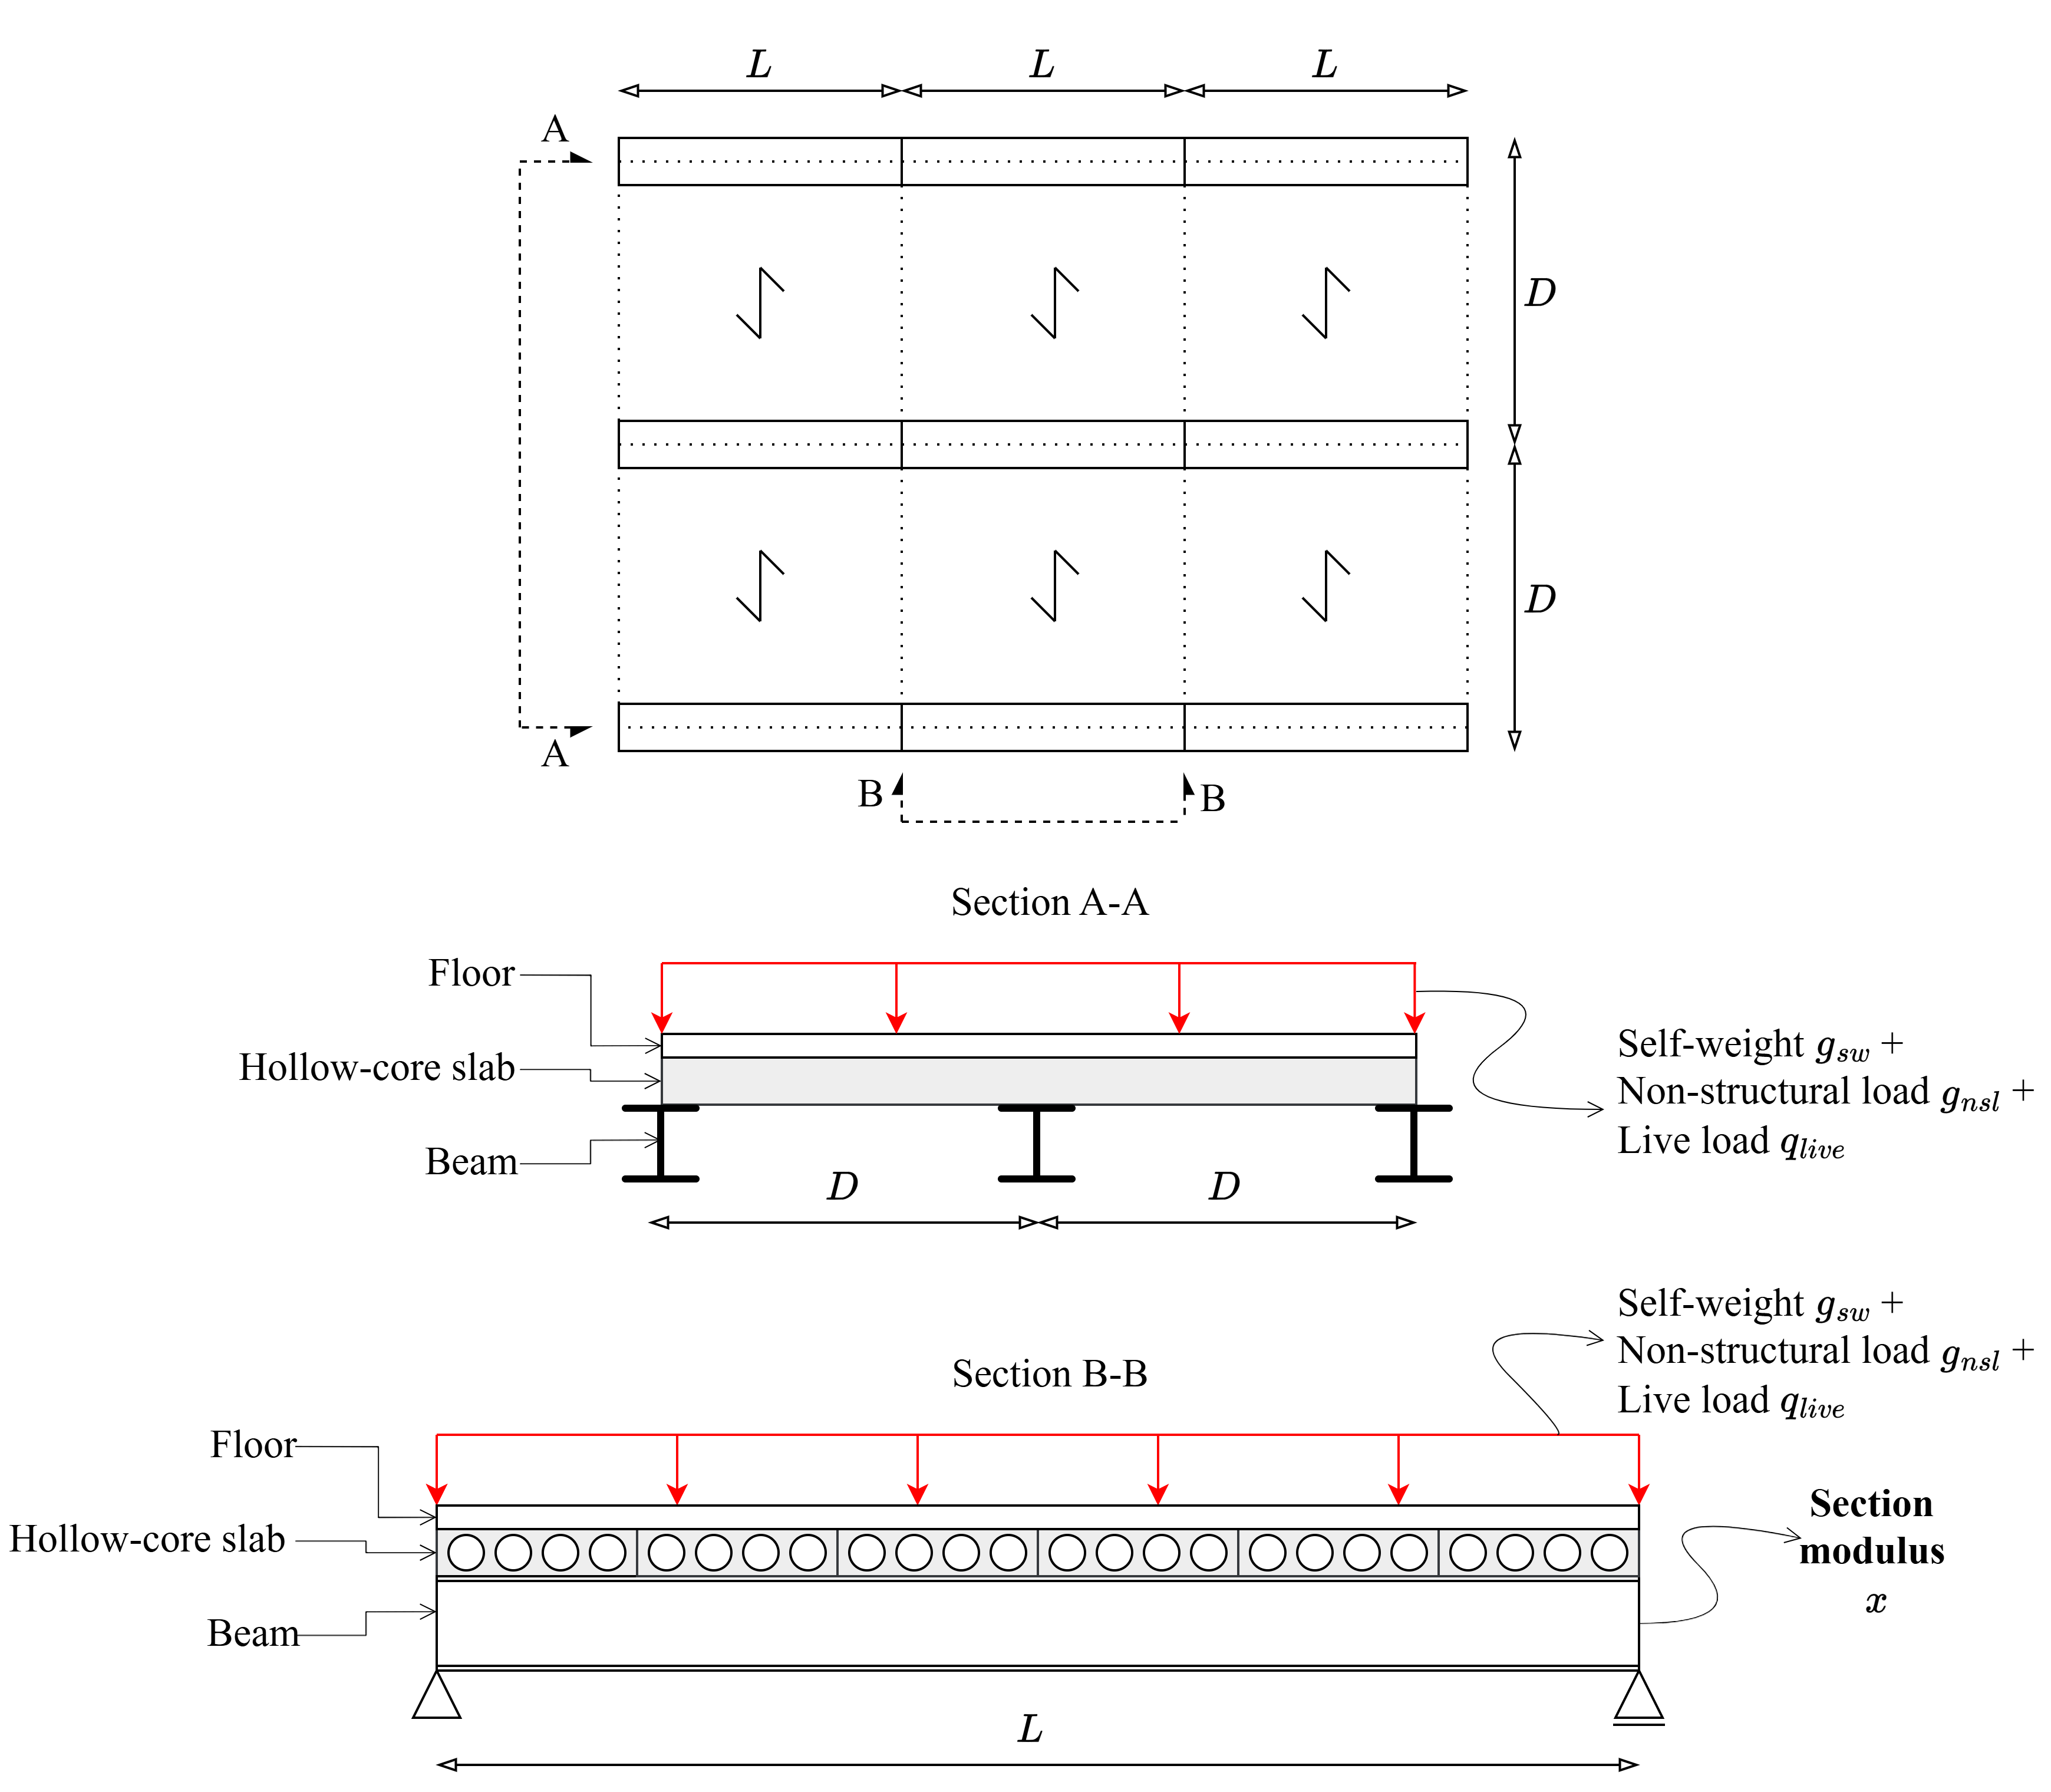
\includegraphics[width=0.8\linewidth]{Images/beam_diagram.png}
    \caption{The typical case study, with the loads, dimensions and decision variable indicated. Not to scale.}
    \label{fig:beam}
\end{figure}

\begin{table}[h]
    \centering
    
    \begin{tabular}{c|c|c|c|c|c}
         Variable & Description & Unit & Distribution & Mean & CoV  \\ \hline
         $q_{live}$& Variable load & kN/m\textsuperscript{2}& Gumbel & 1.2&0.5\\
         $g_{sw}$& Self-weight load& kN/m\textsuperscript{2}& Normal& 4.137& 0.1\\
         $g_{nsl}$& Non-structural load& kN/m\textsuperscript{2}& Normal& 2.8&0.1\\
         $f_y$& Yield strength steel& N/mm\textsuperscript{2}& Lognormal& 282&0.05\\
         $\theta_R$& Resistance model uncertainty&-& Lognormal& 1.225&0.075\\
         $\theta_E$& Load effect model uncertainty&-& Lognormal& 1.0&0.1\\
         $\theta_q$& Live load model uncertainty&-& Lognormal& 1.0&0.1\\
         $L$ & Beam length & m & Deterministic & 12 & - \\
         $D$ & Beam spacing & m & Deterministic & 12 & - \\
         $x$ & Plastic section modulus & mm\textsuperscript{3} & Deterministic & \emph{To be optimised} & - \\
    \end{tabular}
   \caption{Distributions of random variables in the limit state function used in the case study, derived from \citep{Vrouwenvelder2024ReliabilityEurocodes,Hingorani2023TowardsDesign}.} \label{tab:distributions}
\end{table}

\begin{figure}[h]
    \centering
    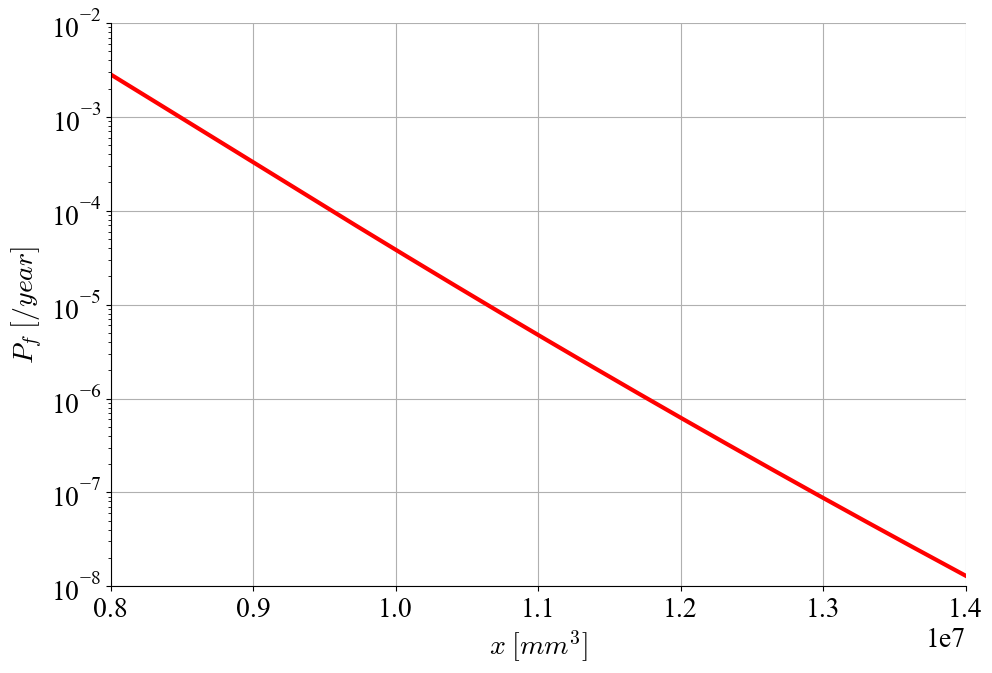
\includegraphics[width=0.7\linewidth]{Images/P_f.png}
    \caption{Failure probability $P_f(x)$}
    \label{fig:P_f}
\end{figure}

The linear formulation for the construction cost and emissions is used, with parameters given in Table \ref{tab:C_E_params}.
The $x$-independent costs $C_0$ and emissions $E_0$ are estimated on indications of labour costs and transport emissions \citep{Knibbe2026PlaceHolder, Musa2024COPeriod, Fortus2025StalenVergunning}.
The values for $C_1$ and $E_1$ are based on an assumed linear relation between the beam mass and section modulus, given in \citep{Hingorani2023SustainabilityDesign}, along with a steel material cost of 2 \EUR{}/kg steel \citep{Hingorani2023SustainabilityDesign, bauforumstahle.V.2026BaukostenBauforumstahl} and emission intensity 1.87 kg CO\textsubscript{2}eq/kg  steel \citep{TATASteel2017BenefitsOwnership}.
As mentioned in Section \ref{sec:appraisal}, using $SWTP \cdot N_f$ as (part of) the additional damage costs $C_H$ is justified. 
In this case, it is assumed that $C_{H,other}$ is negligible compared to this term. 
The number of expected fatalities in the case of failure is estimated at 0.97 \citep{Knibbe2026PlaceHolder, Hingorani2020ConsequenceStructures}, with the SWTP equal to 2.775 million \EUR{} per life saved, resulting in a $C_H$ of 2.70 million \EUR{}.
Finally, the additional failure emissions $E_H$ are derived from the loads carried by the beam, representing the embodied emissions of the floor and other, non-structural components which are replaced in the case of failure \citep{Knibbe2026PlaceHolder, Hingorani2023SustainabilityDesign}.

\begin{table}[]
    \centering
    \begin{tabular}{c|c|c|c}
         Parameter & Description& unit  &value 
\\ \hline
 $C_0$& $x$-independent costs& EUR  &1.00*10\textsuperscript{3} 
\\
 $C_1$& $x$-dependent costs&EUR$/mm^3$ &9.81*10\textsuperscript{-4}
\\
 $C_H$& Additional failure costs&EUR &2.70*10\textsuperscript{6}
\\
 $E_0$& $x$-independent emissions&kg CO\textsubscript{2}eq &3.33*10\textsuperscript{2}
\\
 $E_1$& $x$-dependent emissions&kg CO\textsubscript{2}eq/$mm^3$ &9.17*10\textsuperscript{-4}
\\
 $E_H$& Additional failure emissions&kg CO\textsubscript{2}eq &6.65*10\textsuperscript{4}\\\end{tabular}
    \caption{Parameter values in the cost and emission functions}
    \label{tab:C_E_params}
\end{table}

To find an optimal reliability, several different optimisations are now performed.
First, the cost and emission functions are considered as two separate optimisations, before being combined in a multi-objective optimisation problem.
Next, the primary weighted sum approach is presented, combining the costs and emissions in one objective function.
Finally, the alternative $\varepsilon$-constraint is considered, considering one of the functions as a constraint.

\subsection{Separate objectives}

In this approach, both objective functions are optimised separately.
The result is two optimal values for the design parameter $x$, denoted here as $x_{opt,C}$ and $x_{opt,E}$, and accompanying $\beta_{opt,C}$ and $\beta_{opt,E}$.
Figure \ref{fig:separate} and Table \ref{tab:separate} show the results of this approach.
Both functions have a similar shape, with the optimum of $C_{total}$ located at a larger value of $x$ compared to the optimum of $E_{total}$ (marked by a blue and green star, respectively), making $\beta_{opt,E}$ smaller than $\beta_{opt,C}$ ($P_{f,opt}$ is larger). 
This is caused by the difference in the `push-pull' effect between the two objectives.
The ratio $E_H/E_1$ is smaller for the emissions compared to the equivalent ratio $C_H/C_1$ for the costs, so the optimal failure probability considering emissions is `pushed' upwards relative to the cost-optimal failure probability, which has a stronger `pull' downwards.
In the next steps, values between the two optima will be considered.

\begin{figure}[h!]
    \centering
    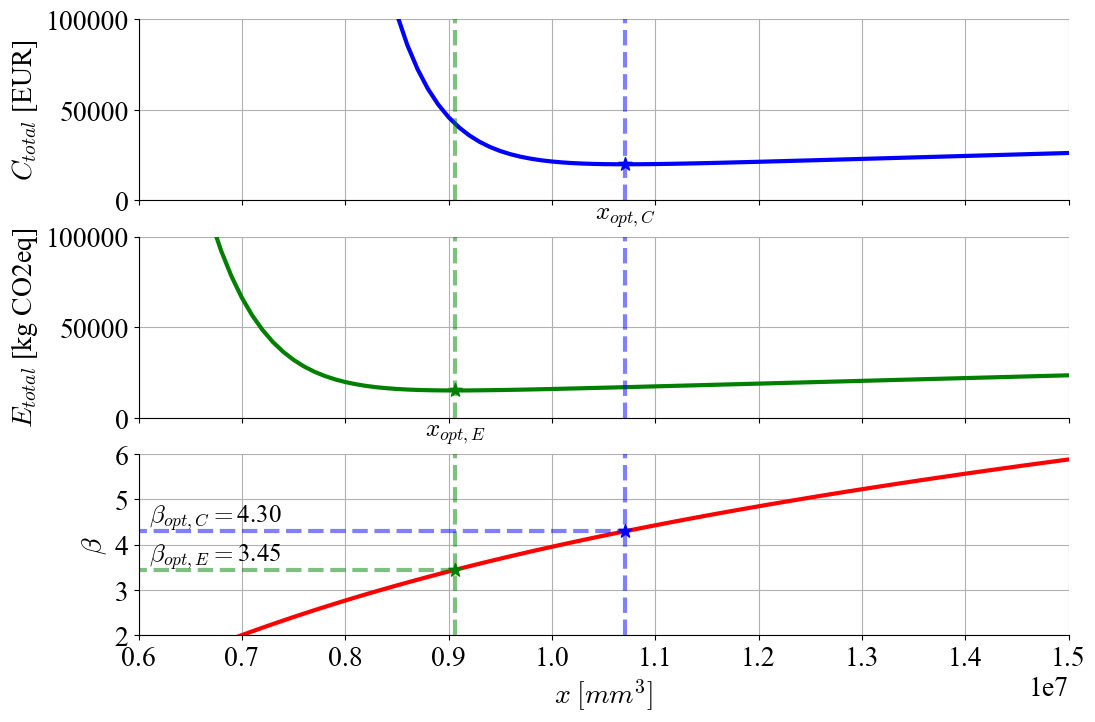
\includegraphics[width=0.95\textwidth]{Images/demo_separate.png}
    \caption{Separate optimisation of the two costs and emissions.}
    \label{fig:separate}
\end{figure}



\begin{table}[h]
    \centering
    \begin{tabular}{c|c|c|c}
         &   $C_{tot}$ optimal&$E_{tot}$ optimal &Unit\\ \hline
         $x_{opt}$& 
     $1.07*10^7$&$9.06*10^6$ &mm\textsuperscript{3}\\
 $C_{tot}$& 19,966&42,213 &$\EUR{}$\\
 $E_{tot}$& 16,951&15,129 &kg CO\textsubscript{2}eq\\
 $P_{f,opt}$& $8.7*10^{-6}$&$2.8*10^{-4}$ &/year\\
 $\beta_{opt}$& 4.30&3.45 &yearly\\\end{tabular}
    \caption{Results of the separate optimisation of the two objective functions}
    \label{tab:separate}
\end{table}


% \newpage
\subsection{Multi-objective}

Now, a multi-objective optimisation problem is considered.
Both objectives are minimised simultaneously, resulting in a Pareto front: a set in the objective space of the problem that contains all combinations of objective function values that are attainable for some value of $x$, and are \emph{non-dominated}: no other value of $x$ yields an improvement (decrease, in this case) in both objectives simultaneously \citep{Deb2001Multi-objectiveAlgorithms, Martins2021EngineeringOptimization}.
In a two-objective problem, the Pareto front visualises a trade-off in objective space: the curve shows how much one would need to be sacrificed for an improvement in the other.

In this specific problem, the Pareto front can be found given the separate results from the previous approach. 
In between the separate optima, one objective increases while the other decreases.
Outside of this region, marked by the dashed lines in Figure \ref{fig:separate}, both objectives increase
Any point in the objective space found by using a value of $x$ outside the range $[x_{opt,E},x_{opt,C}]$ is thus dominated by a point within this range.
In other words, the Pareto front consists of all combinations of $C_{total}$ and $E_{total}$ found by simply varying $x$ from $x_{opt,E}$ to $x_{opt,C}$
The result is given in Figure \ref{fig:pareto}.
The stars again represent the separate optima of the two objectives, and the curve connecting them represents values found using any $x$ located in between the optima.

Note that the axes in Figure \ref{fig:pareto} are not equally scaled: the difference in $C_{total}$ at both ends of the curve is much larger than the difference in $E_{total}$.
This can also be determined from the shapes of the objective functions in Figure \ref{fig:separate} and the values of the objective function in Table \ref{tab:separate}: the region enclosed by the separate optima contains the steep part of $C_{total}$ (dominated by the failure cost term), and the shallow part of $E_{total}$ (dominated by the construction and obsolescence terms).
Moving $x$ from the cost-optimum to the emission-optimum will reduce $E_{total}$ approximately linearly, while $C_{total}$ increases much more sharply.
In other words, the more emissions are reduced, the more expensive (in terms of increased cost) further reduction becomes.
To determine the final optimal reliability, only one objective function can be optimised.
The next step presents the primary method for this, as proposed, by combining both objective functions through shadow-costing.


\begin{figure}[h!]
    \centering
    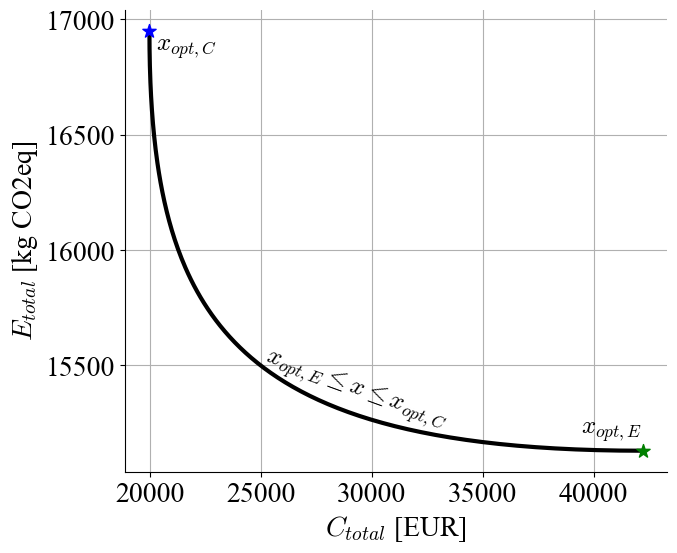
\includegraphics[width=0.7\textwidth]{Images/demo_pareto.png}
    \caption{Pareto front of the two objectives.}
    \label{fig:pareto}
\end{figure}

\subsection{Weighted sum approach / shadow costing}

The two objectives are combined into a single, augmented cost function using a shadow price $c_e$ of 0.8 euros per kilogram of CO\textsubscript{2}-equivalent emissions, which corresponds with values found in current literature \citep{EuropeanInvestmentBank2025ShadowPricing, KamaliSaraji2024BridgingApplications, Wang2017TheIndustry,  WorldBank2025PriceDashboard}.
As mentioned, this value is difficult to quantify, so the effect of different shadow prices will be investigated in the next section.

Figure \ref{fig:single} presents the single-objective optimisation, and Table \ref{tab:single} contains the numerical results, along with those from Table \ref{tab:separate} for comparison.
For a shadow cost of 0.8 \EUR{}/kg CO\textsubscript{2}eq, the optimal reliability index reduces by 0.12 with respect to the monetary optimum.
Comparing these results to the target reliability values given in ISO2394 (Table G.4) \citep{iso2394}, buildings of this consequence with `medium relative safety costs' have a target reliability of 4.2, with `small' costs increasing it to 4.4.
The monetary optimum $\beta_{opt,C}$ lies in between these two values, while the augmented optimum $\beta_{opt,aug}$ is slightly smaller than the medium value.
Therefore, for a shadow cost of 0.8 $\EUR{}$/kg CO\textsubscript{2}eq, the optimal reliability changes by `one half cost class.'


\begin{figure}[h!]
    \centering
    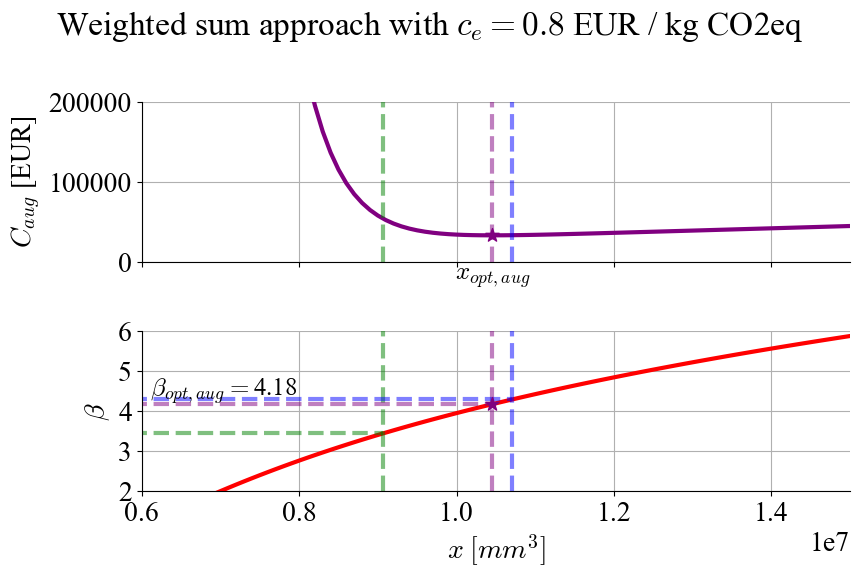
\includegraphics[width=0.85\textwidth]{Images/demo_single.png}
    \caption{Single-objective optimisation of the augmented cost function. The locations of the separate optima are indicated by dashed lines; blue for $\beta_{opt,C}$, green for $\beta_{opt,E}$, purple for $\beta_{opt,aug}$.}
    \label{fig:single}
\end{figure}

\begin{table}[]
    \centering
    \begin{tabular}{c|c|c|c}
         &   $C_{tot}$ optimal&$E_{tot}$ optimal &$C_{aug}$ optimal\\ \hline
         $x$& 
     $1.07*10^7$&$9.06*10^6$
&$1.05*10^{7}$\\
 $C_{tot}$& 19,966&42,213
&20,100\\
 $E_{tot}$& 16,951&15,129
&16,578\\
 $C_{aug}$& 33,527& 54,316&33,362\\
 $P_f$& $8.7*10^{-6}$&$2.8*10^{-4}$
&$1.5*10^{-5}$\\
 $\beta_{opt}$& 4.30&3.45&4.18\\\end{tabular}
    \caption{Results of the separate optimisation of the two objective functions}
    \label{tab:single}
\end{table}

\newpage
\subsection{$\varepsilon$-constraint approach}

As mentioned, the shadow price $c_e$ is not the only option to derive a single optimum from the two objective functions; either one can also be formulated as a constraint to the other.
To formulate the threshold values of these constraints, $E_{max}$ and $C_{max}$, the monetary optimum is considered as a reference point.
A relative desired reduction in emissions $\delta E_{desired}$ or an allowed relative increase in costs $\delta C_{allowed}$ is mandated with respect to this reference.
The problem is then formulated as:
\begin{equation}
    \begin{aligned}
        \min_{x} \quad & C_{total}(x)\\
        \textrm{s.t.} \quad & E_{total}(x) \leq E_{max} = (1 - \delta E_{desired}) \cdot E_{total}(x_{opt,C}) \\
    \end{aligned}
\end{equation}
Or:
\begin{equation}
    \begin{aligned}
        \min_{x} \quad & E_{total}(x)\\
        \textrm{s.t.} \quad & C_{total}(x) \leq C_{max} = (1 + \delta C_{desired}) \cdot C_{total}(x_{opt,C})\\
    \end{aligned}
\end{equation}
Figure \ref{fig:constrain} contains the results of this alternative approach, for different relative decreases in emissions and increases in costs.
The minimum of $E_{tot}$ is approximately 11\% smaller than the emissions at $x_{opt,C}$ (see Table \ref{tab:separate}), so this is the upper bound of $\delta E_{desired}$.
Similarly, a $\delta C_{allowed}$ up to 111\% is considered. 
In general, increasing $\delta E_{desired}$ or $\delta C_{allowed}$ decreases the constrained optimal reliability index.
For $\beta_{copt,Emax}$, this decrease appears linear for small  $\delta E_{desired}$, but becomes sharper for larger values. 
For $\beta_{copt,Cmax}$, an opposite pattern appears: the decrease is sharp for small allowed cost increases, but levels off for larger values.
This corresponds to the aforementioned shape of the separate functions in Figure \ref{fig:separate}, now connected to the reliability index: the more emissions are reduced, the more expensive reducing them becomes, \emph{as does the reduction in the optimal reliability index}.

\begin{figure}[h!]
    \centering
    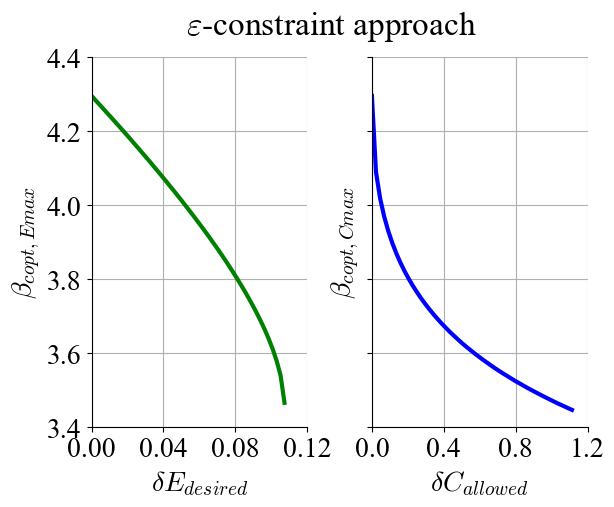
\includegraphics[width=0.6\textwidth]{Images/demo_constraint.png}
    \caption{Optimal reliability found through the $\varepsilon$-constraint approach, varying with relative contraint thresholds}
    \label{fig:constrain}
\end{figure}

% \begin{table}
%     \centering
%     \begin{tabular}{c|c|c|c|c}
%  & \multicolumn{4}{c}{$\delta E_{desired}$ w.r.t. monetary optimum}\\ \hline
%          &  0\%&  1\%&  5\%&  10\% \\ \hline
%          $x$&  $1.07*10^7$&  $1.06*10^7$&  $1.01*10^7$&  $9.37*10^6$\\
%          $C_{tot}$&  19,966&  19,990&  20,921&  30,262 \\
%          $E_{tot}$&  16,951&  16,781&  16,103&  15,256\\
%          $P_f$&  $8.7*10^{-6}$&  $1.1*10^{-5}$&  $3.0*10^{-5}$&  $1.5*10^{-4}$\\
%          $\beta_{copt,Emax}$&  4.30&  4.24&  4.01&  3.62\\
%     \end{tabular}
%     \caption{Results of optimising the cost function with a relative reduction in emissions as constraint}
%     \label{tab:E_constr}
% \end{table}


% \begin{table}
%     \centering
%     \begin{tabular}{c|c|c|c|c|c}
%  & \multicolumn{5}{c}{$\delta C_{allowed}$ w.r.t. monetary optimum}\\ \hline
%          &  0\%&  1\%&  5\%&  10\%& 20\%\\ \hline
%          $x$&  $1.07*10^7$
% &  $1.04*10^7$&  $1.01*10^7$&  $9.93*10^6$& $8.71*10^6$\\
%          $C_{tot}$&  19,966
% &  20,165&  20,962&  21,961& 23,958\\
%          $E_{tot}$&  16,951
% &  16,506&  16,090&  15,848& 15,585\\
%          $P_f$&  $8.7*10^{-6}$
% &  $1.6*10^{-5}$&  $3.1*10^{-5}$&  $4.5*10^{-5}$& $7.1*10^{-5}$\\
%          $\beta_{copt,Cmax} $&  4.30&  4.15&  4.01&  3.92& 3.81\\
%     \end{tabular}
%     \caption{Results of optimising the emission function with a relative increase in costs as constraint}
%     \label{tab:C_constr}
% \end{table}



\newpage
\section{Analysis}

In this section, the results of the case study are analysed to investigate the influence of different aspects on the optimal reliability indices, and the difference in result between the conventional and proposed approach.
First, the effect of different values for the shadow price is considered, and a connection is made between the two multi-objective approaches.
Next, the effect of varying the coefficients of variation in the probabilistic model of the structure and the additional damage costs $C_H$ on the optimal reliabilities is investigated, followed by a number of variants of the considered structure derived from \cite{Hingorani2023SustainabilityDesign}.
Finally, the ratio between the steel material cost and shadow-costed emissions is considered.
All these aspects are expected to influence the optimal reliability values indices, but the effect on the difference in results between the conventional and proposed augmented approaches is harder to predict.
This is represented by the difference between the conventional optimal reliability $\beta_{opt,C}$ and the augmented value $\beta_{opt,aug}$, here denoted as $\Delta \beta$:
\begin{equation}
    \label{eqn:delta_beta}
    \Delta \beta = \beta_{opt,C} - \beta_{opt,aug}
\end{equation}

\subsection{Shadow price $c_e$}

If the optimal reliability takes account of both cost and emissions, it is intuitively located between the optimal values of the separate objectives.
In the weighted sum approach, its location is governed by the shadow price: the larger $c_e$, the more $x_{opt,aug}$ moves from $x_{opt,C}$ towards $x_{opt,E}$, and the smaller $\beta_{opt,aug}$ becomes, so $\Delta \beta$ increases.

The effect of different shadow prices on the augmented optimal reliability is visualised in Figure \ref{fig:single_ce}, where the value of $\beta_{opt,aug}$ is plotted against the value of $c_e$.
The left panel shows the effect of a range of shadow prices generally found in literature, between 0 and 1 \EUR{} per kg CO\textsubscript{2}eq \citep{EuropeanInvestmentBank2025ShadowPricing, KamaliSaraji2024BridgingApplications, Wang2017TheIndustry,  WorldBank2025PriceDashboard}.
The right panel shows the theoretical effect of very large shadow prices, which would cause $\beta_{opt,aug}$ to approach $\beta_{opt,E}$, as the costs become negligible in $C_{aug}(x)$ compared to the emissions.
As noted, the shadow price can be interpreted in different ways.
Intuitively, it could be viewed as a literal price to be paid for emitted carbon, set through regulation or market mechanisms.
Alternatively, it could also be interpreted more abstractly, as a relative importance of emissions with respect to cost, independent of actual pricing.
If hypothetically, the emission reduction were considered more important than cost minimisation, an arbitrarily large value of $c_e$ could be used.
For consistency, in the remaining analyses a shadow price of 0.8 \EUR{}/kg CO\textsubscript{2}eq will be used as in the original case study.

For this and other more commonly found shadow prices, the effect on the optimal reliability index remains of similar order to the difference between target reliabilities between different combinations of cost and consequence classes given in ISO2394 \citep{iso2394}.
Thus, the reduction in $\beta_{opt}$ with respect to the monetary optimum, $\Delta \beta$, can be considered equal to a `partial class' for the range of shadow prices found in literature.
This could potentially be amplified by differential discounting \citep{Emmerling2019TheEmissions, Nestico2023AImpacts}, which would likely increase the additional `push' from the shadow-costed emissions with respect to the costs.

\begin{figure}[h!]
    \centering
    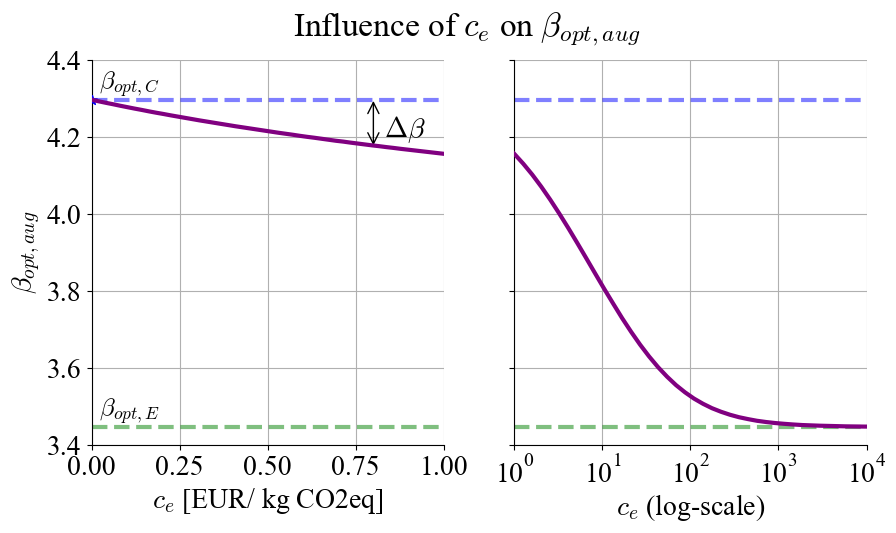
\includegraphics[width=0.7\textwidth]{Images/demo_ce.png}
    \caption{Augmented optimum dependent on shadow price. The left panel shows the effect for small but more realistic values of $c_e$, while the right panel shows how the optimal reliability approaches $\beta_{opt,E}$ for very large shadow prices.}
    \label{fig:single_ce}
\end{figure}

The weighted sum and $\varepsilon$-constraint approach can be connected through the Pareto front of Figure \ref{fig:pareto}.
Every point on this front is associated with a value for the shadow price $c_e$, a desired decrease in emissions $\Delta E_{desired}$ or allowed cost increase $\Delta C_{allowed}$ (which can be derived from the relative changes $\delta E_{desired}$ or $\delta C_{allowed}$).
This connection is visualised in Figure \ref{fig:triangle}: a constraint formulated with respect to the monetary optimum `cuts off' part of the Pareto front with either too much increase in costs or too little reduction in emissions.
The cut-off point in the remaining Pareto front then becomes the constrained optimum for the other objective.
Furthermore, the slope of the Pareto front at this point is then the reciprocal of the shadow costs, or equivalently, a line perpendicular to the Pareto front at this point has a slope equal to $c_e$.
This relation between the slope of a Pareto front and weight factors used in a weighted sum approach is a well-known phenomenon in multi-objective optimisation \cite{Deb2001Multi-objectiveAlgorithms}, and could be utilised to understand how the value of the shadow cost $c_e$, desired emission reduction $\delta E_{desired}$, or allowed cost increase $\delta C_{allowed}$ all interact with the value of the two objective functions and optimal reliability.


\begin{figure}[h!]
    \centering
    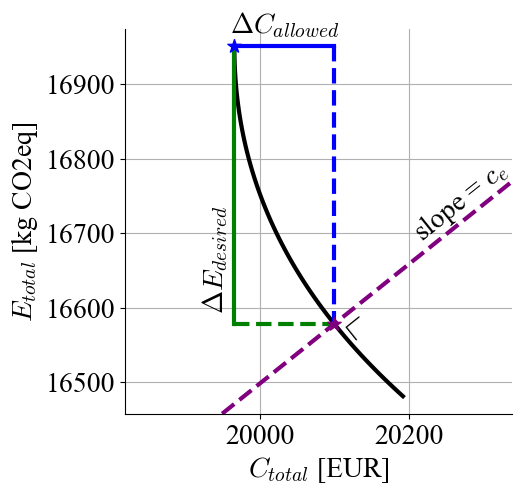
\includegraphics[width=0.55\textwidth]{Images/demo_triangle.png}
    \caption{Geometric interpretation of the shadow price, emission reduction and cost increase on the Pareto front}
    \label{fig:triangle}
\end{figure}


By considering that every point on the Pareto front of Figure \ref{fig:pareto} can be connected to a value of $\beta_{opt,aug}$.
Figure \ref{fig:single_3d} shows this connection: the reliability index $\beta$ corresponding to each value of $x$ in the region of interest is plotted as a curve hovering over the Pareto front associated with the same values of $x$.
For increasing $c_e$, $\delta E_{desired}$ or $\delta C_{allowed}$, the optimum moves along the Pareto front, starting at the blue star representing the costs-only optimum ($c_e = 0$), and moving towards the green star representing the emissions-only optimum ($c_e \rightarrow \infty$).
The costs at the optimum increase while the emissions decrease, and the optimal reliability $\beta_{opt,aug}$ `slides' downwards along the curve above the Pareto front.

\begin{figure}[h!]
    \centering
    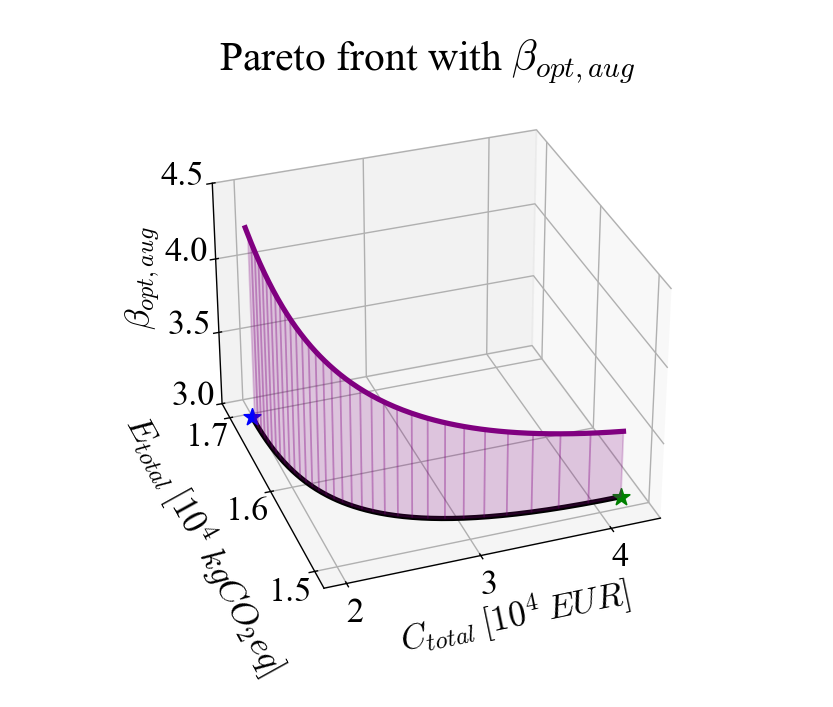
\includegraphics[width=0.7\textwidth]{Images/demo_3d.png}
    \caption{Visualisation of the interaction between the two objectives and the optimal reliability.}
    \label{fig:single_3d}
\end{figure}

For either of the optimisation approaches, some quantity needs to be chosen to find a single optimum from a two-objective problem, either a shadow price $c_e$ or a threshold value $C_{max}$ or $E_{max}$ setting a constraint.
The Pareto front connecting the two separate optima cannot, by itself, be used to find a single optimum.
However, its shape can be used to inform the choice of this quantity using the visualisations.
Which approach works best can depend on the local context and legislation, and in some cases, this may help choose the parameter value directly.
If a comprehensive `carbon tax' is active, this gives an intuitive choice for $c_e$.
If there is a general target for emission reduction, for the construction sector or for the economy in general, this could inform $\delta E_{desired}$, especially if the `status quo' based on monetary optimisation is used as a reference.
Finally, if some amount of money needs to be allocated for emission reductions, this can be used to set $\delta C_{allowed}$.

\clearpage
\subsection{Coefficients of variation}

An important aspect influencing the optimal reliability is the degree of uncertainty in the considered structure.
In general, the larger the variability of the loads and resistances, the larger $P_f$ is for a constant $x$.
This means a larger $x$ is needed to achieve the same reliability, so the cost of increasing safety effectively becomes larger (the `push' increases), leading to a smaller $\beta_{opt}$.
To investigate this effect in this case study, the three values of $\beta_{opt}$ for the considered beam are recalculated with differing coefficients of variations for three important variables in the limit state function: the yield strength $f_y$, permanent loads $g_{sw}$ and $g_{nsl}$, and live load $q_{live}$.
These are denoted as $V_f$, $V_g$ (for both permanent loads) and $V_q$, and were initially set to 0.05, 0.10 and 0.50 respectively \citep{Knibbe2026PlaceHolder, Hingorani2023SustainabilityDesign}.
Adjusting these values means the probabilistic model no longer follows the relevant background literature \citep{JCSS2000ProbabilisticDesign, Vrouwenvelder2024ReliabilityEurocodes}, so this should be considered as an academic exercise not representative of a real structure.
The adjusted coefficients of variation have therefore been chosen, somewhat arbitrarily,
The weighted sum approach is followed, keeping the shadow price $c_e$ at 0.8 \EUR{}/kg CO\textsubscript{2}eq.

Figure \ref{fig:cov} contains the result of this exercise.
As expected, larger coefficients of variation lead to smaller optimal reliabilities and vice versa.
% For the chosen values, the largest deviation from the values found using the original coefficients of variations is approximately 0.06 (the bottom line of Figure \ref{fig:cov}), half of the original difference found between $\beta_{opt,C}$ and $\beta_{opt,aug}$ using $c_e=0.8$.
Remarkably, $\Delta \beta$ is consistent across the different sets of coefficients of variation.
It appears that the reduction in optimal reliability with respect to the monetary optimum is unaffected by the degree of variability in the probabilistic model of the structure.
% As mentioned, this result can be linked to the constrained approach through the Pareto front.
% A similar analysis with a chosen value for $\delta E_{desired}$ or $\delta C_{allowed}$ would return identical results and is therefore not performed here.

\begin{figure}[h!]
    \centering
    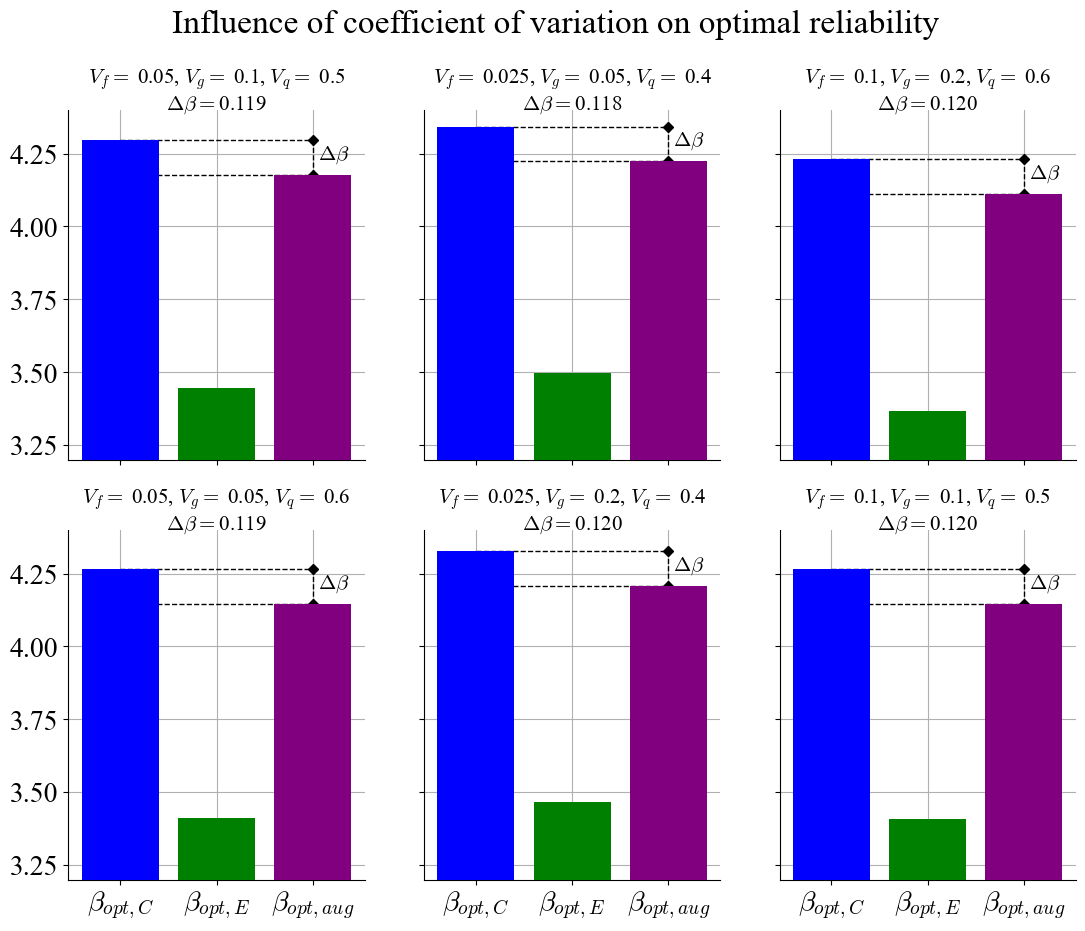
\includegraphics[width=0.85\textwidth]{Images/demo_cov_2.png}
    \caption{Influence of the coefficients of variation of the yield strength $V_f$, permanent load $V_g$, and live load $V_q$ pn the optimal reliability indices. A shadow price of 0.8 \EUR{}/kg CO\textsubscript{2}eq  has been used to find $\beta_{opt,aug}$}
    \label{fig:cov}
\end{figure}


\subsection{Damage costs $C_H$}

Next, the influence of the damage costs $C_H$ on the result is investigated.
As mentioned in Section \ref{sec:appraisal}, this value should include the term $SWTP \cdot N_f$ to represent human life risk, and a possible additional term $C_{H,other}$ to represent other indirect damage.
This latter term was originally neglected in the case study, as the material damage cost outside replacement of the beam is likely orders of magnitude smaller than the life risk costs for an office building.
However, it is worthwhile to investigate how hypothetical large values of $C_{H,other}$ would influence the optimal reliability, and especially the difference between the conventional and augmented optimum $\Delta \beta$.
For that reason, Figure \ref{fig:CH} presents $\beta_{opt,C}$ and $\beta_{opt,aug}$ varying across different orders of magnitude for the total $C_H$ ($\beta_{opt,E}$ is ignored here, as it is not influenced by $C_H$), including values smaller than $SWTP \cdot N_f$.
Again, this should be viewed as an academic exercise.

Both optimal reliability indices with increasing $C_H$, which is expected as the `pull' effect is strengthened.
Both appear to increase logarithmically with $C_H$, which is consistent with literature performing similar analyses \citep{Fischer2019OptimalDesign, Rackwitz2000OptimizationVerification}.
Notably, $\Delta \beta$ is constant once again.
It appears that the value of $C_H$, like the coefficients of variation, also does not influence the impact of the shadow costed emissions.


\begin{figure}[h!]
    \centering
    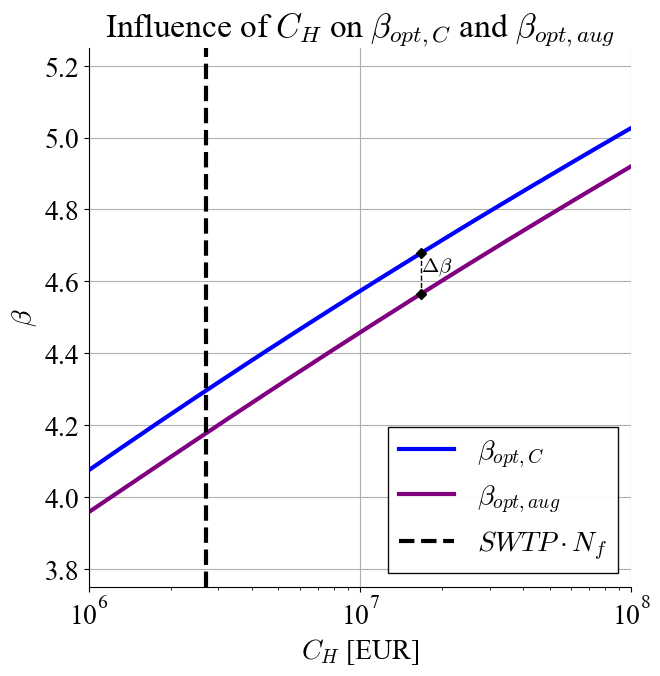
\includegraphics[width=0.65\textwidth]{Images/demo_C_H_sens.png}
    \caption{Optimal reliabilities dependent on the additional damage costs $C_H$. A shadow price of 0.8 \EUR{}/kg CO\textsubscript{2}eq has been used to find $\beta_{opt,aug}$}
    \label{fig:CH}
\end{figure}
\clearpage
\subsection{Variation of structure parameters}

The paper this case study has been adapted from \citep{Hingorani2023SustainabilityDesign} considered different variants of the considered structure by varying several parameters in the design problem: the beam length $L$, beam spacing $D$ underneath the floor slabs, the characteristic yield strength $f_{y,k}$, and two load ratios; $a_q$ setting the variable load $q_{live,k}$ to the total load $g_{sw,k} + g_{nsl,k} + q_{live,k}$, and $a_g$ setting the self-weight $g_{sw}$ to the permanent load $g_{sw,k} + g_{nsl,k}$ (all formulated in terms of characteristic values, which influence the mean values in the probabilistic model).
These variations resulted in a `population' of 50 different feasible designs (more details can be found in \cite{Hingorani2023SustainabilityDesign}).
To further investigate the generalisability of the case study results presented in the current work, the same optimisations have been performed on this population, resulting in 50 different values of $\beta_{opt,C}$, $\beta_{opt,E}$, $\beta_{opt,aug}$ (given $c_e=$0.80 \EUR{}/CO\textsubscript{2}eq), and the derived $\Delta \beta$.
Figure \ref{fig:population} and Table \ref{tab:population_stats} display the empirical cumulative distribution functions (CDF) and general statistics of these results.

All three optimal reliability indices are reasonably constant across the different variants, with the environmental optimum having somewhat more variance than the other two.
This is likely caused by the additional failure emissions $E_H$ which depend on both the floor are supported by the beam, set by the length $L$ and spacing $D$, as well as the load ratios $a_q$ and $a_g$.
The additional failure costs, $C_H$, depend only on the floor area and not the load ratios, hence this parameter varies to a lesser degree across the different variants in the population than $E_H$, and so does its `pull' effect on the respective optimal reliability.

The distribution of the augmented optimal reliability appears similar to that of the monetary optimum, shifted approximately 0.12 to the left.
This corresponds to the value of $\Delta \beta$ found in the original case study, which is also rather stable across this population of variants.
From this analysis, it appears that $\Delta \beta$ is reasonably consistent across different variants of the same structure, in terms of supported area, characteristic load ratios and material strength.


\begin{figure}[h!]
    \centering
    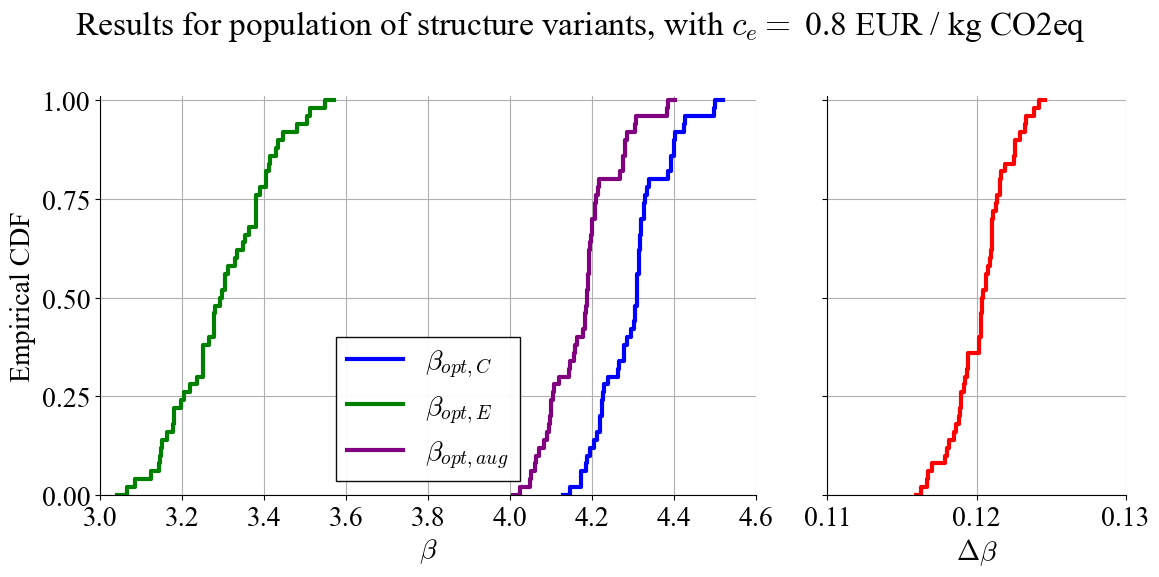
\includegraphics[width=0.85\textwidth]{Images/demo_population.png}
    \caption{Empirical cumulative distribution of optimal reliabilities (left) and $\Delta \beta$ (right) for a population of structure variants. A shadow price of 0.8 \EUR{}/kg CO\textsubscript{2}eq has been used to find $\beta_{opt,aug}$ and $\Delta \beta$}
    \label{fig:population}
\end{figure}

\begin{table}[]
    \centering
    \begin{tabular}{c|c|c|c|c}
         &  $\beta_{opt,C}$ & $\beta_{opt,E}$&$\beta_{opt,aug}$ &$\Delta \beta$\\ \hline
         Min& 
     4.15& 3.07&4.02 &0.116\\
 Median& 4.31& 3.30&4.19 &0.120\\
 Max& 4.50& 3.55&4.38 &0.124\\
 Mean& 4.30& 3.30&4.18 &0.120\\
 Std.dev.& 0.0815& 0.1161&0.083 &0.00185\\
 CoV& 0.019& 0.035&0.020 &0.015\\\end{tabular}
    \caption{Statistics of the optimal reliability indices of the population of structure variants}
    \label{tab:population_stats}
\end{table}

\subsection{Relation emission to material cost}

It has been shown that both the conventional and augmented optimal reliability indices are sensitive to the coefficients of variation, failure costs, and structural parameters.
However, $\Delta \beta$ is not affected as much, instead being determined by the shadow price $c_e$ as Figure \ref{fig:single_ce} shows.
An alternative view can be adopted by considering the shadow price and emissions of the structural material in relation to its monetary cost.
An \emph{emission-cost ratio} can then be defined as $c_e \cdot E_1 / C_1$ (unitless), and for the final analysis of this section, the effect of this ratio on $\Delta \beta$ is investigated.
A reasonable range for this ratio has been estimated based on various sources for the steel price \citep{bauforumstahle.V.2026BaukostenBauforumstahl, Bouwenmetstaal2024CostComponents, BritishConstructionalSteelworkAssociationCostSteelConstruction.info}, embodied emission of steel \citep{TATASteel2017BenefitsOwnership, WorldSteelAssociation2021ClimateSteel, OveArupPartners2023BuildingsSteel}, and carbon shadow price \citep{WorldBank2025PriceDashboard, EuropeanInvestmentBank2025ShadowPricing, Wang2017TheIndustry}.

Figure \ref{fig:ratio} shows the result.
A similar analysis has also been performed considering a reinforced concrete beam under the floor instead of a steel profile.
The parameters of this alternative case study are given in 

This is similar to the analysis behind Figure \ref{fig:single_ce}, where the shadow price $c_e$ was varied and the `pull'-term $c_e (E_{const}(x) + E_H) \frac{P_f(x)}{\gamma}$ in $E_{total}$ also changes.
Here, the focus is on the `push'-effect is varied in both objective functions, but the result is similar: $\Delta \beta$ increases approximately linearly with the emission-cost ratio.
The interpretation is different, however: while $c_e$ can (as mentioned) be considered a general weight factor representing the relative importance of the two objective functions in their entirety, the emission-cost ratio represents the environmental impact of the specific structural material relative to its monetary costs.
This is an important distinction, especially when considering the impact of the proposed approach across different structures.
If one structure is relatively cheap (low $C_1$) but emission-intensive (larger $E_1$) compared to another, it would have a larger emission-cost ratio and the proposed augmented optimisation would thus result in a larger $\Delta \beta$, even if the shadow price $c_e$ applied in both optimisations is the same.
It is then not the relative weight of emissions in general, but the difference in environmental impact relative to cost \emph{for the specific structure} that determines how the optimal reliability should change when emissions are considered.

\begin{figure}[h!]
    \centering
    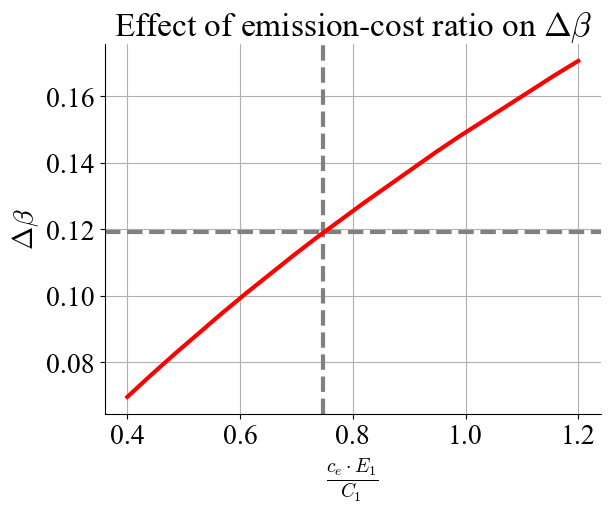
\includegraphics[width=0.65\textwidth]{Images/demo_ratio.png}
    \caption{$\Delta \beta$ as a function of the unitless ratio between shadow-costs and monetary costs of steel. The initial ratio and its outcome are marked.}
    \label{fig:ratio}
\end{figure}

Concrete version

emissions based on \citep{InformationsZentrumBetonGmbH2023BetonEPD-IZB-20230328-IBG1-DE}, 0.078 kgCO2 / kg C30 concrete
cost based on \citep{UniconPRICE2024}, 0,104 UER / kg C30 concrete
\newpage
\section{Conclusion}

This paper proposed and demonstrated an augmented method to establish optimal reliabilities for engineering structures, which allows decision makers to take social and environmental sustainability into account.
In terms of social sustainability, it was concluded that monetarisation of potential fatalities due to structural failure can be ethically justified, and is in fact needed to ensure the optimal reliability criterion provides value in addition to the existing acceptance criterion.
This can be incorporated without fundamentally changing the approach, but was not explicitly mandated previously.

In terms of environmental sustainability, a larger alteration to the conventional approach was proposed, by incorporating emissions in the optimisation problem using a lifetime emission model based on the Rackwitz renewal model that the cost function is also based on.
This similarity still allows the proposed method to be integrated well into existing codes.
These two models can be combined into a single, augmented cost function using a shadow price for emissions, which can then be optimised to find an augmented optimal reliability.
Alternatively, a constrained optimisation problem can be formulated, where one model forms the cost function and the other the constraint.

In a typical case study, the result of these two optimisation approaches is compared to the conventional method.
Optimising the costs and emissions separately yields two optimal criteria, with the emissions leading to a smaller optimal value.
Using a combined objective function with a shadow price of 0.80 \EUR{}/ kg CO\textsubscript{2}eq, the optimal reliability index reduces by 0.12, though this is influenced by the applied shadow price value $c_e$.
A larger value yields a larger reduction, as does a larger desired emission reduction $\delta E_{desired}$ or allowed cost increase $\delta C_{allowed}$ in the alternative approach.
The two approaches interact through the Pareto front, where a value needs to be chosen for either $c_e$, $\delta E_{desired}$ or $\delta C_{allowed}$, leading to an optimal reliability index in between the monetary optimum $\beta_{opt,C}$ and emission minimum $\beta_{opt,E}$.
The optimal reliabilities are affected by the degree of uncertainty in the probabilistic model of the considered structure, as well as the additional damage costs $C_H$, and structure parameters such as the supported floor area, load ratios and yield strength.
The difference between the conventional and augmented methods appears to be mostly unaffected by these, however, and is mainly driven by the importance of the emissions relative to the costs, described either through the shadow price $c_e$ in general or the emission shadow cost relative to the monetary cost of the specific structure.

% Subsequently, the sensitivity of this result to the shadow price of the emissions with the costs was investigated.
% By considering the problem as different types of optimisation problems, the influence of this important parameter was shown.
% The larger the shadow price, the smaller the augmented optimal reliability becomes, though the difference is modest for the range of values commonly found in literature.
% The alternative approach was also demonstrated by formulating the constraint based on a relative desired decrease in emissions or allowed increases in costs.
% To obtain an optimal reliability value from combining the two models, either a shadow price or a threshold value for a constraint is needed.
% Finally, the influence of the additional damage costs $C_H$ were shown, including some deliberation on the role of human life safety in this aspect.
% It was concluded that using this value can be ethically justified, even if some trepidations still exist.
% In general, the optimal reliability value is very sensitive to the value of $C_H$, hence its use in defining consequence classes

% The proposed framework is able to establish optimal reliability values taking both

\subsection*{CRediT authorship contribution statement}

\textbf{Jelle Knibbe}: Conceptualisation, Formal analysis, Writing – original draft
\textbf{Raphaël Steenbergen}: Conceptualisation, Writing – review \& editing
\textbf{Pieter van Gelder}: Writing – review \& editing
\textbf{Amir Pooyan Afghari}: Writing – review \& editing

\subsection*{Acknowledgement}
This paper is part of a PhD project supported by Delft University of Technology (TU Delft) and Netherlands Organisation for Applied Scientific Research (TNO).

\bibliography{references.bib}

%% The Appendices part is started with the command \appendix;
%% appendix sections are then done as normal sections
\appendix

% \newpage

\section{Alternative case study: concrete beam}

The alternative case study still considers a beam supporting a hollow-core slab floor in an an office building.
However, this is now a reinforced concrete beam, with the effective beam depth as the decision parameter $x$, see Figure \ref{fig:beam_concrete} below.
This problem was adapted from \citep{Hingorani2025Resource-EfficientConcepts}, with data on material cost and emissions gathered from \citep{UniconPRICE2024}.

\begin{figure}[h]
    \centering
    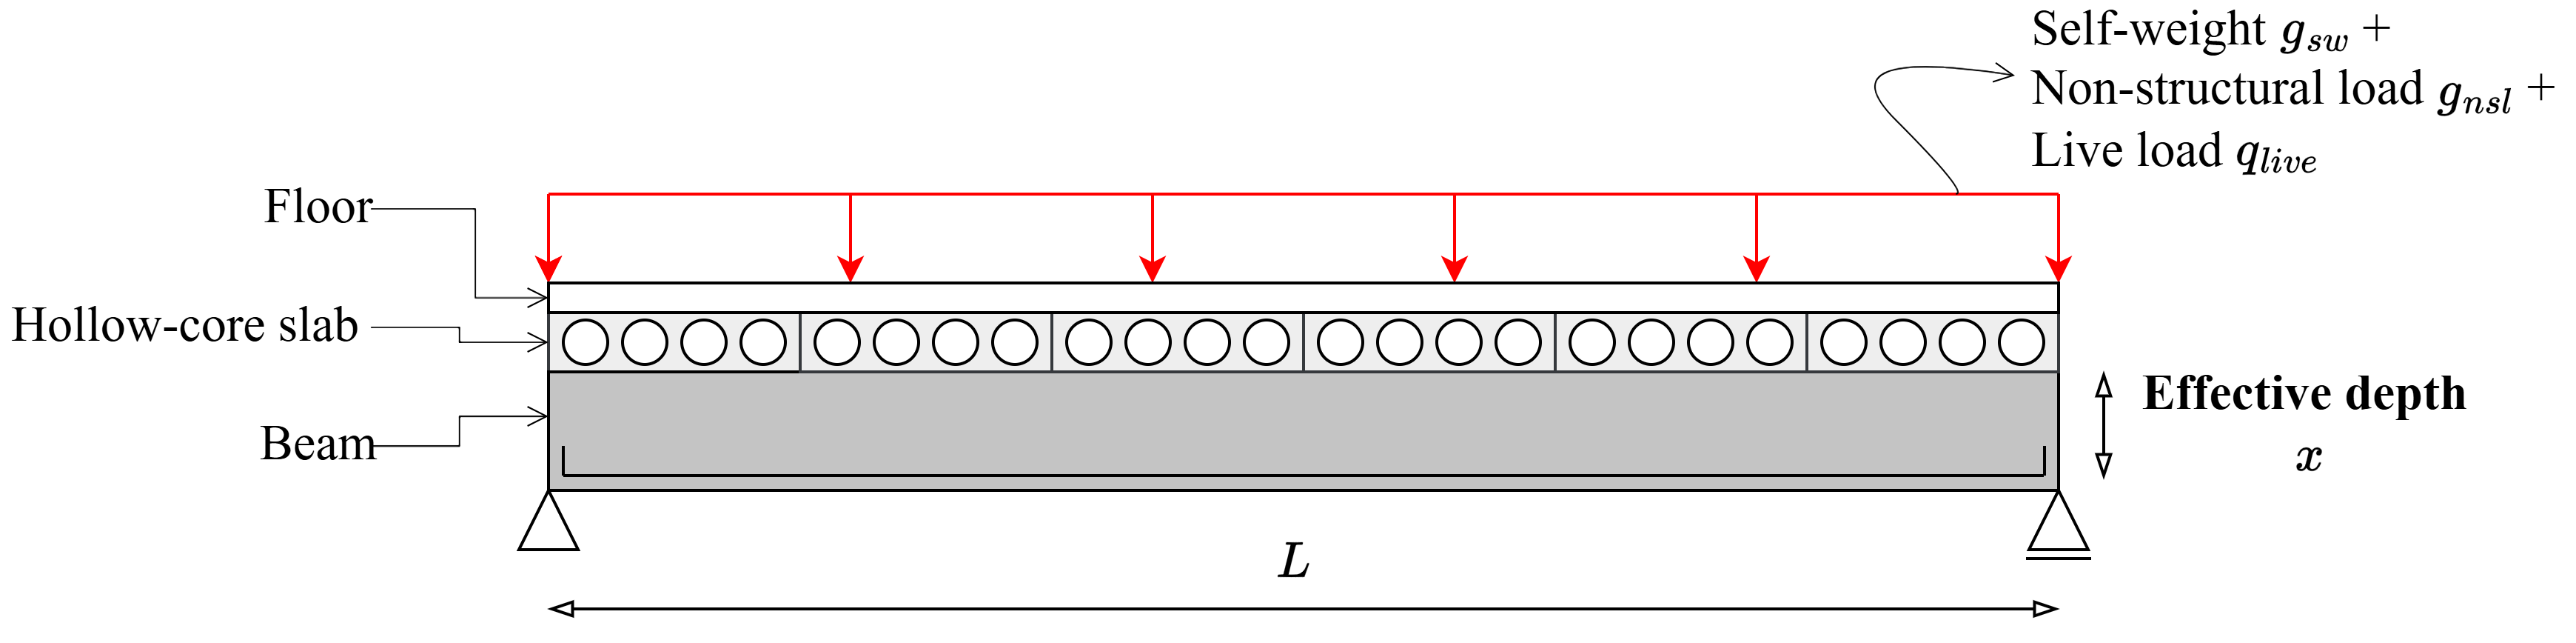
\includegraphics[width=0.8\linewidth]{Images/beam_concrete_variant.png}
    \caption{The alternative case study, with the loads, dimensions and decision variable indicated. Not to scale.}
    \label{fig:beam_concrete}
\end{figure}

The limit state function for the bending failure mechanism of this structure is:

\begin{equation}
    \label{eqn:LSF_alt}
    Z = \theta_R b \rho_s x^2 f_y \left( 1 - \frac{1}{2} \rho_s \frac{f_y}{f_c} \right) - \theta_E \frac{(g_{sw} + g_{nsl} + \theta_q q_{live})DL^2}{8}
\end{equation}

With $b$ the beam width and $\rho_s$ the reinforcement ratio, both deterministic, while the reinforcement yield strength $f_y$ and concrete compressive strength $f_c$ (class C30/37) are stochastic variables.
The other parameters are identical to Equation \ref{eqn:LSF}, though the distribution of the resistance model uncertainty $\theta_R$ has been adjusted to the specific resistance model.
The full probabilistic model of this structure is described in Table \ref{tab:distributions_concrete}.
The parameter values of the cost and emission functions are given in Table \ref{tab:C_E_params_concrete}.
The `push'-parameters $C_1$ and $E_1$ are again based on a linear relation between the decision variable and beam volume, with a material cost of $\EUR{}$ 0.10/kg concrete, and emission intensity of 0.11 kg CO\textsubscript{2}eq/kg concrete.
Note that the parameter $E_1$ is adjusted to adhere to the emission-cost ratio for which this alternative case study is considered.
The $x$-independent variables $C_0$ and $E_0$ are based on the same assumptions as for the original steel variant of the case study, with a small increase to account for the concrete volume below the effective depth of the beam (based on an assumed concrete cover of 30 mm, independent of $x$).
Finally, the 'pull' parameters $C_H$ and $E_H$ are identical to the original steel variant of the case study.

\begin{table}[h]
    \centering
    
    \begin{tabular}{c|c|c|c|c|c}
         Variable & Description & Unit & Distribution & Mean & CoV  \\ \hline
         $q_{live}$& Variable load & kN/m\textsuperscript{2}& Gumbel & 1.2&0.5\\
         $g_{sw}$& Self-weight load& kN/m\textsuperscript{2}& Normal& 4.137& 0.1\\
         $g_{nsl}$& Non-structural load& kN/m\textsuperscript{2}& Normal& 2.8&0.1\\
         $f_y$& Yield strength reinforcement steel& N/mm\textsuperscript{2}& Lognormal& 538.4&0.045\\
 $f_c$& Concrete compressive strength& N/mm\textsuperscript{2}& Lognormal& 35.4&0.1\\
         $\theta_R$& Resistance model uncertainty&-& Lognormal& 1.035&0.07\\
         $\theta_E$& Load effect model uncertainty&-& Lognormal& 1.0&0.1\\
         $\theta_q$& Live load model uncertainty&-& Lognormal& 1.0&0.1\\
         $L$ & Beam length & m & Deterministic & 12 & - \\
         $D$ & Beam spacing & m & Deterministic & 12 & - \\
 $b$& Beam width& mm& Deterministic & 500&-\\
 $\rho_s$& Reinforcement ratio& -& Deterministic & 0.05&-\\
         $x$& Effective beam depth& mm& Deterministic & \emph{To be optimised} & - \\
    \end{tabular}
 \caption{Distributions of random variables in the limit state function used in the concrete variant of the case study, derived from \citep{Vrouwenvelder2024ReliabilityEurocodes,Hingorani2023TowardsDesign}.}   \label{tab:distributions_concrete}
\end{table}

\begin{table}[h]
    \centering
    \begin{tabular}{c|c|c|c}
         Parameter & Description& unit  &value 
\\ \hline
 $C_0$& $x$-independent costs& EUR  &1.05*10\textsuperscript{3}\\
 $C_1$& $x$-dependent costs&EUR$/mm^3$ &1.60*10\textsuperscript{-5}\\
 $C_H$& Additional failure costs&EUR &2.70*10\textsuperscript{6}
\\
 $E_0$& $x$-independent emissions&kg CO\textsubscript{2}eq &3.84*10\textsuperscript{2}\\
 $E_1$& $x$-dependent emissions&kg CO\textsubscript{2}eq/$mm^3$ &1.78*10\textsuperscript{-5}\\
 $E_H$& Additional failure emissions&kg CO\textsubscript{2}eq &6.65*10\textsuperscript{4}\\\end{tabular}
    \caption{Parameter values in the cost and emission functions for the concrete variant of the case study}
    \label{tab:C_E_params_concrete}
\end{table}


% \section{Example Appendix Section}
% \label{app1}

% Appendix text.

% %% For citations use: 
% %%       \cite{<label>} ==> [1]

% %%
% Example citation, See \cite{lamport94}.

%% If you have bib database file and want bibtex to generate the
%% bibitems, please use
%%
% \bibliographystyle{elsarticle-num} 


%% else use the following coding to input the bibitems directly in the
%% TeX file.

%% Refer following link for more details about bibliography and citations.
%% https://en.wikibooks.org/wiki/LaTeX/Bibliography_Management

% \begin{thebibliography}{00}

% %% For numbered reference style
% %% \bibitem{label}
% %% Text of bibliographic item

% \bibitem{lamport94}
%   Leslie Lamport,
%   \textit{\LaTeX: a document preparation system},
%   Addison Wesley, Massachusetts,
%   2nd edition,
%   1994.

% \end{thebibliography}
\end{document}

\endinput
%%
%% End of file `elsarticle-template-num.tex'.
